% Type of the document
\documentclass{beamer}

% elementary packages:
\usepackage{graphicx}
\usepackage[latin1]{inputenc}
\usepackage[T1]{fontenc}
\usepackage[english]{babel}
\usepackage{listings}
\usepackage{xcolor}
\usepackage{eso-pic}
\usepackage{mathrsfs}
\usepackage{url}
\usepackage{amssymb}
\usepackage{amsmath}
\usepackage{animate}
\usepackage{multirow}
\usepackage{hyperref}
\usepackage{booktabs}
%\usepackage[demo]{graphicx}
\usepackage{subfig}
%\usepackage{tabularx}
%\usepackage{pgfplotstable}
% recommended:
%\usepackage{booktabs}
%\usepackage{array}
\usepackage{colortbl}

% additional packages
\usepackage{bbm}

% packages supplied with ise-beamer:
\usepackage{cooltooltips}
\usepackage{colordef}
\usepackage{beamerdefs}
\usepackage{lvblisting}
\definecolor{LightCyan}{rgb}{0.88,1,1}
% Change the pictures here:
% logobig and logosmall are the internal names for the pictures: do not modify them. 
% Pictures must be supplied as JPEG, PNG or, to be preferred, PDF
\pgfdeclareimage[height=4.5cm]{logobig}{LogoIRTG}
% Supply the correct logo for your class and change the file name to "logo". The logo will appear in the lower
% right corner:
\pgfdeclareimage[height=0.7cm]{logosmall}{figures/coauthorship}

% Title page outline:
% use this number to modify the scaling of the headline on title page
\renewcommand{\titlescale}{1.0}
% the title page has two columns, the following two values determine the percentage each one should get
\renewcommand{\titlescale}{1.0}
\renewcommand{\leftcol}{0.6}

% Define the title.Don't forget to insert an abbreviation instead 
% of "title for footer". It will appear in the lower left corner:
\title[Network]{Network Centrality}
% Define the authors:
\authora{Ya Qian}
\authorb{Wolfgang Karl H\"ardle}
\authorc{}

% Define any internet addresses, if you want to display them on the title page:
\def\linka{lvb.wiwi.hu-berlin.de}
\def\linkb{\\case.hu-berlin.de}
\def\linkc{\\irtg1792.hu-berlin.de}
% Define the institute:
\institute{Ladislaus von Bortkiewicz Chair of Statistics\\
C.A.S.E. -- Center for Applied Statistics\\
and Economics\\
Humboldt-Universit\"at zu Berlin\\}

% Comment the following command, if you don't want, that the pdf file starts in full screen mode:
\hypersetup{pdfpagemode=FullScreen}

%Start of the document
\begin{document}

% create the title slide, layout controlled in beamerdefs.sty and the foregoing specifications
\frame[plain]{
\titlepage
}

\section{Motivation}
%\frame{
%\frametitle{Network is Everywhere}
%\begin{figure}
%\begin{center}
%\includegraphics[scale=0.15]{Full-Network-Region-Degree-Fruchterman-Reingold-12K-4000x4000-1024x1024.jpg}%\vspace{-0.5cm}
%\caption{Climate Change Network} %\hspace{2cm}
%\href{http://www.pacificrisa.org/projects/social-network-analysis/full-network/}{\textbf{http://www.pacificrisa.org}}
%\end{center}
%\end{figure}
%}


\frame{
\frametitle{International Trade Network}
\begin{figure}
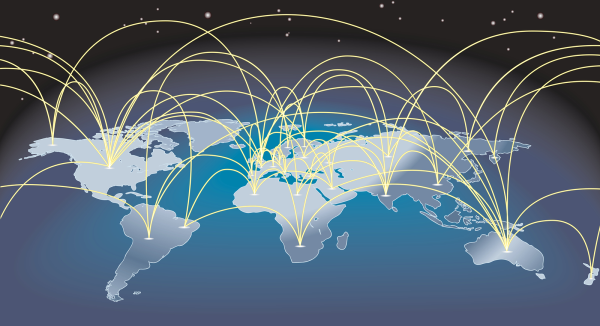
\includegraphics[scale=0.35]{figures/worldtrade}
\caption{International trade picture}
\bigskip
\scriptsize{
\href{http://www.fshcc.com/florida-international-trade-articles/bid/101346/Global-Trade-is-Big-Business-in-Florida}{From Florida State Hispanic Chamber of Commerce}}
\end{figure}
}

\frame{
\frametitle{Production Network}
\begin{figure}
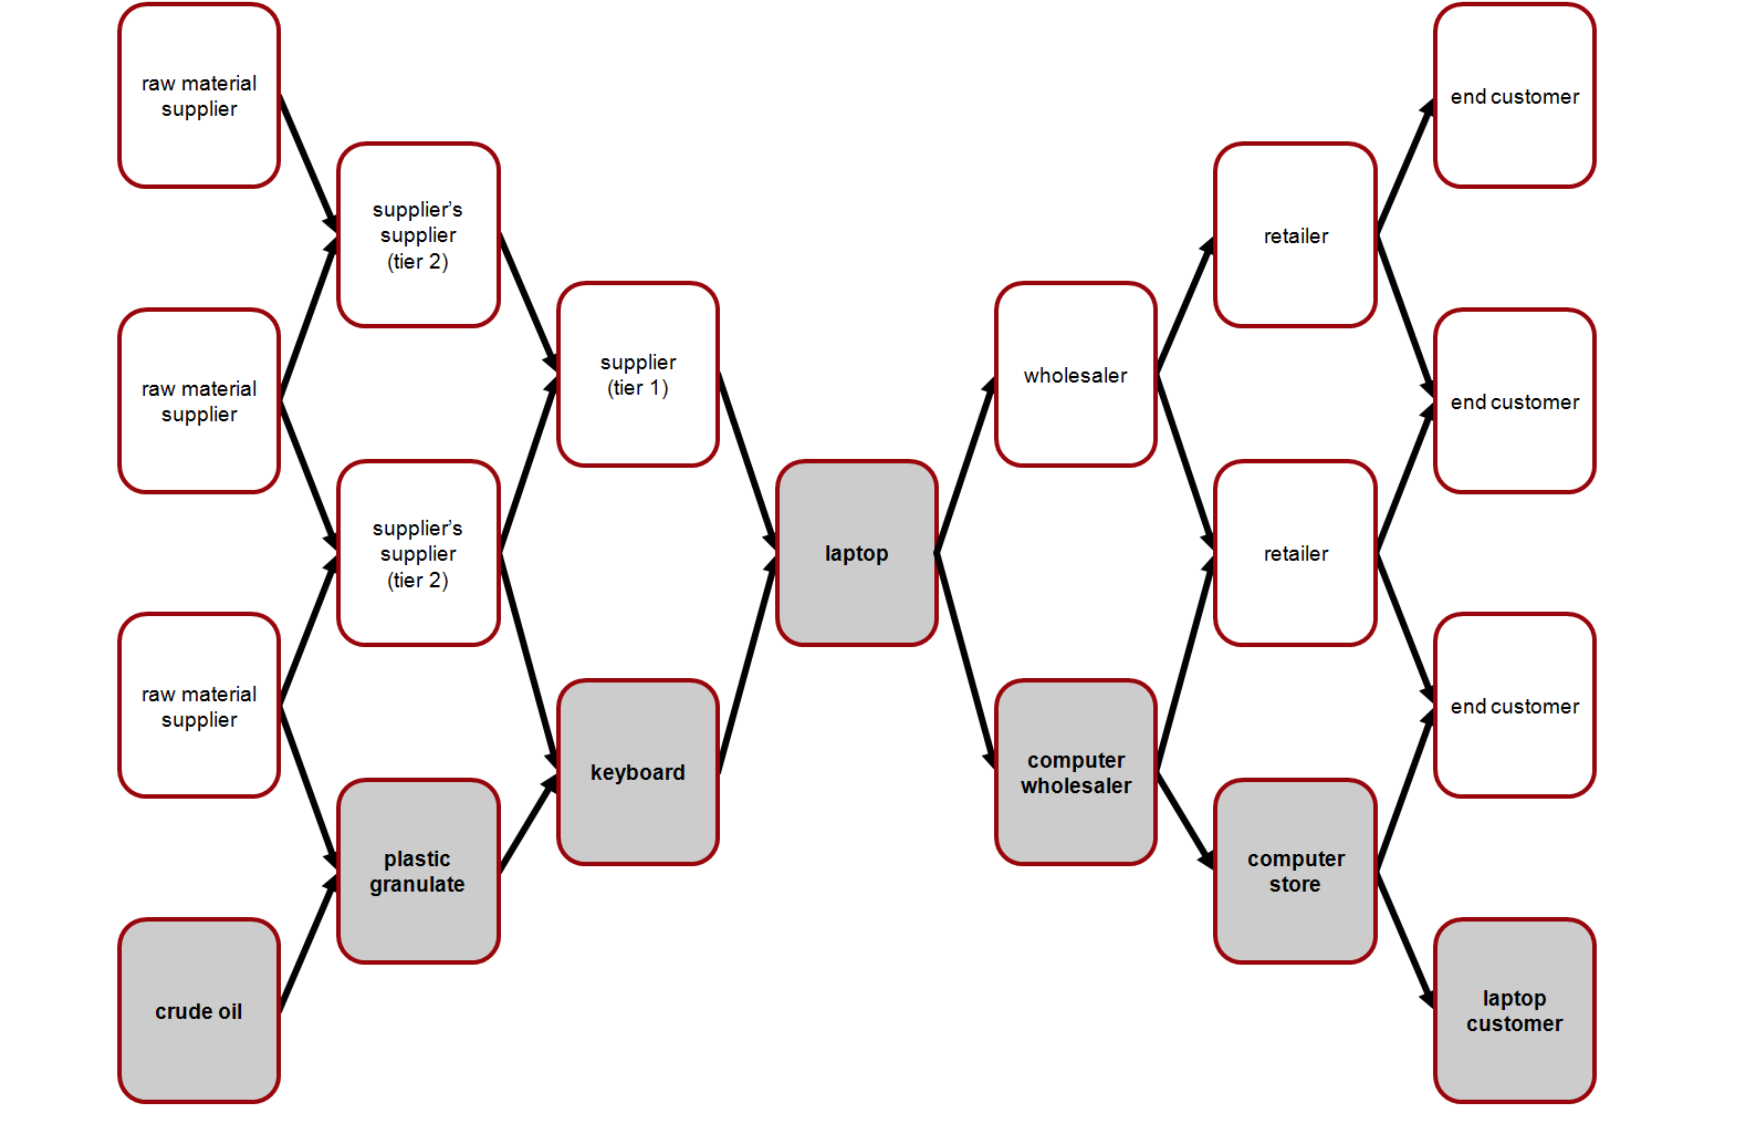
\includegraphics[scale=0.25]{figures/supplychain}
\caption{Supply chain}
\bigskip
\scriptsize{
\href{https://en.wikipedia.org/wiki/Supply_chain}{From Wikipedia}}
\end{figure}
}


\frame{
\frametitle{Social Network}
\begin{figure}
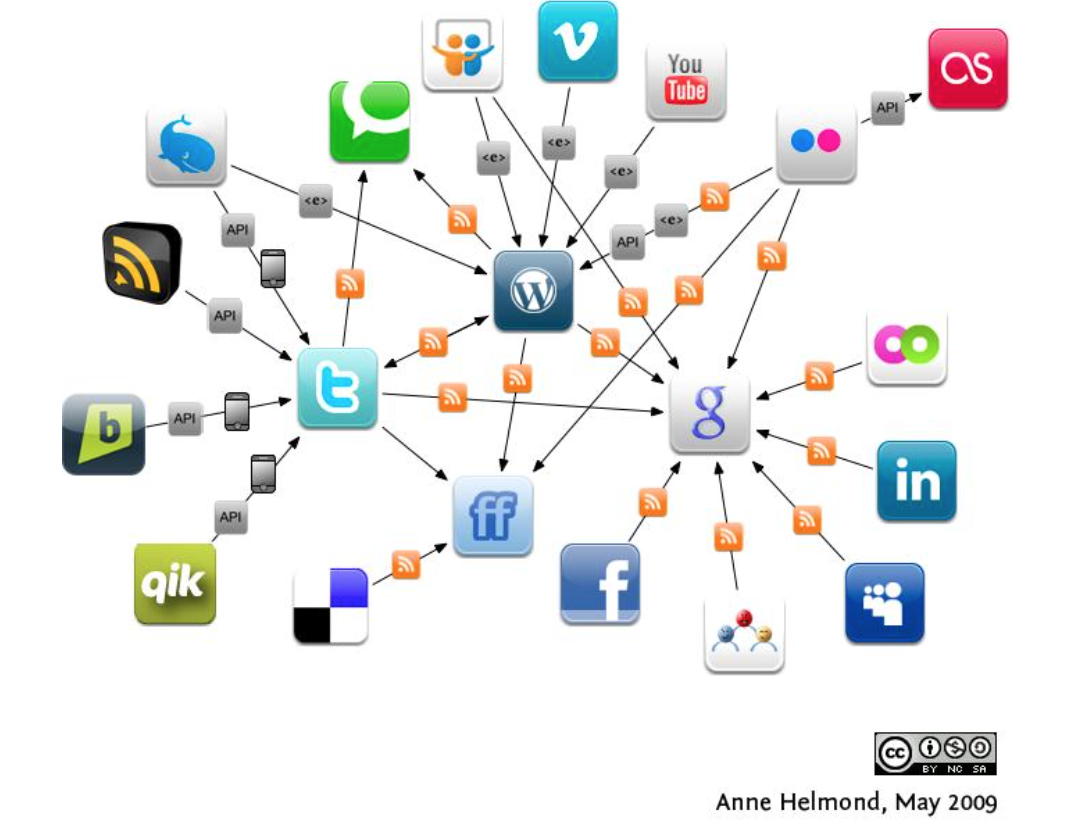
\includegraphics[scale=0.25]{figures/socialnetworks}
\caption{A sample of social network}
\bigskip
\scriptsize{
\href{http://kikolani.com/becoming-accessible-social-networking-social-media.html}{From Webpage Kikolani}}
\end{figure}
}

\frame{
\frametitle{International Financial Network}
\begin{figure}
\includegraphics[scale=0.25]{figures/INFinancialnet}
\caption{A sample of international financial network}
\bigskip
\scriptsize{
From Frank Schweitzer, et al. (Science 325, 422 (2009))}
\end{figure}
}

\frame{
\frametitle{Network of Coauthorship}
\begin{figure}
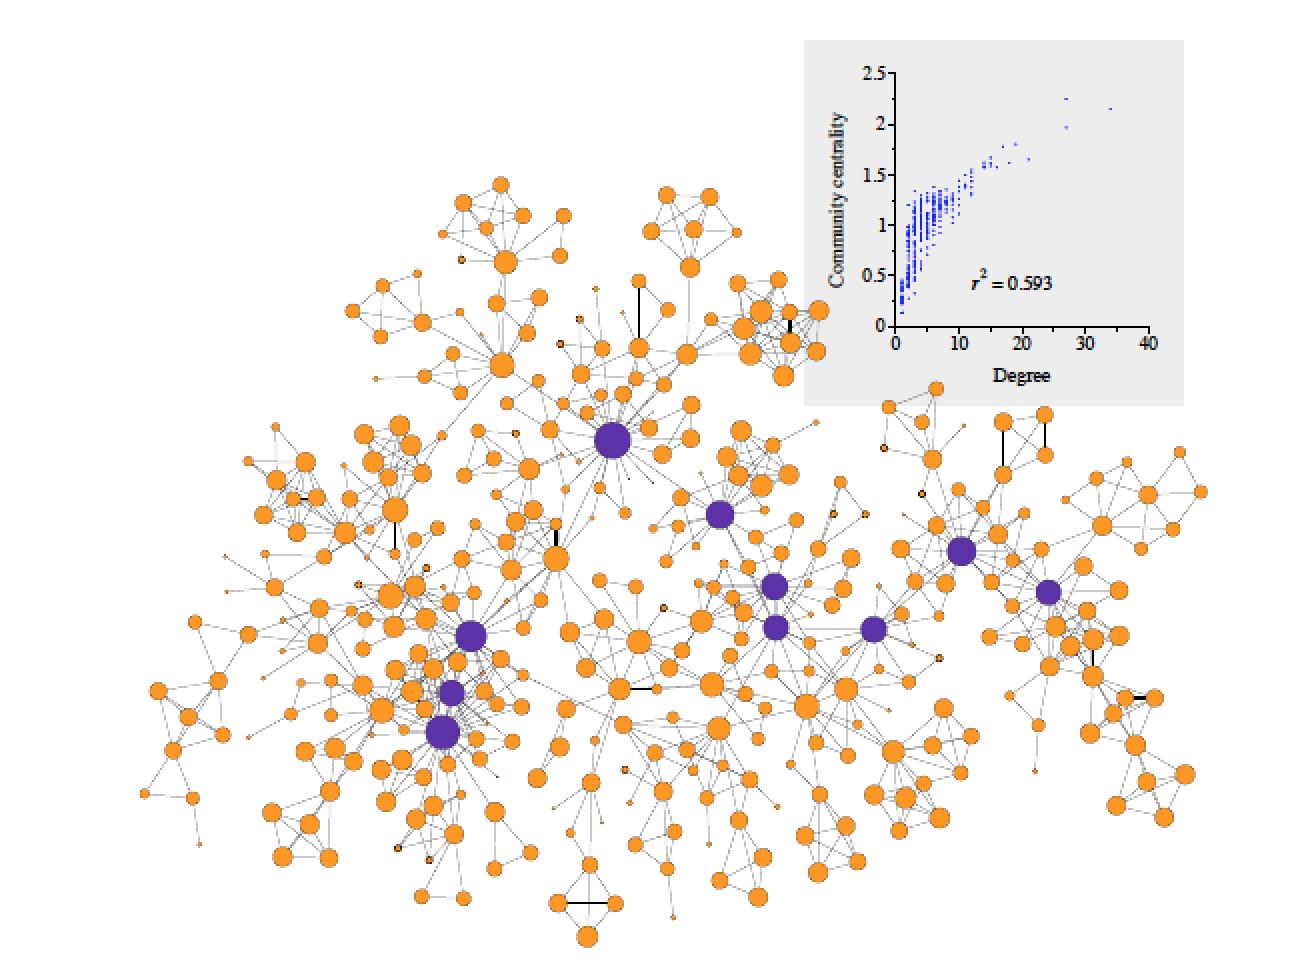
\includegraphics[scale=0.25]{figures/coauthorship}
\caption{A network of coauthorships between 379 scientists whose research centers on the properties of networks of one kind or another}
\bigskip
\scriptsize{
From M.E.J. Newman (Phys. Rev. E 74, 036104 (2006))}
\end{figure}
}

\frame{
\frametitle{A More Specific Coauthorship Graph}
\begin{figure}
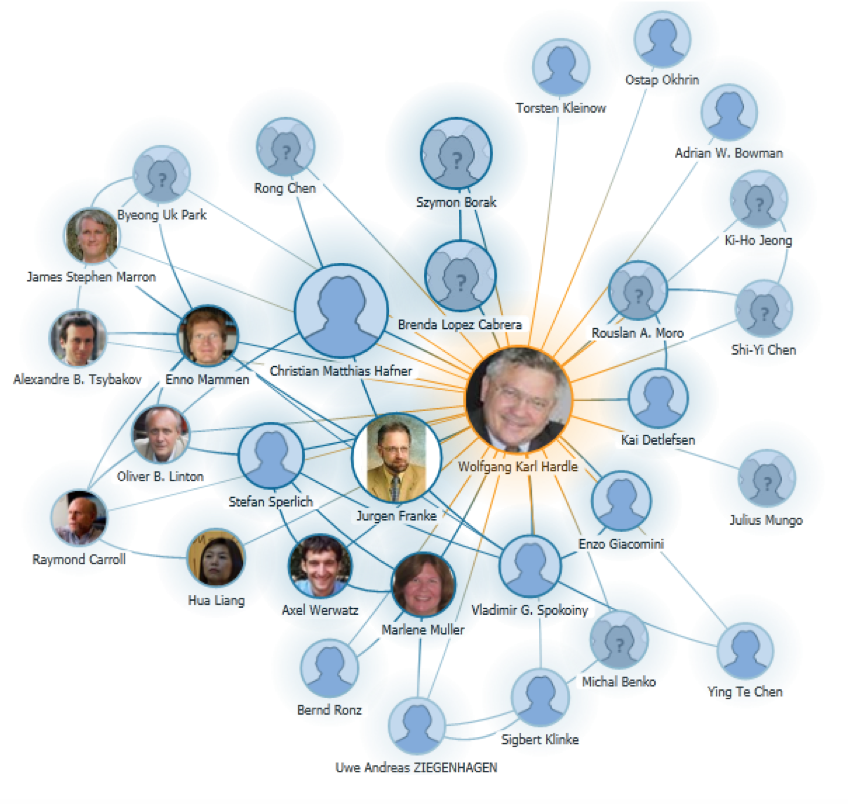
\includegraphics[scale=0.34]{figures/coauthorgraph.png}
\caption{Coauthorship graph of W.K. H\"ardle}
\bigskip
\scriptsize{
\href{http://academic.research.microsoft.com/VisualExplorer\#12530409}
{Source: Microsoft Academic}}
\end{figure}
}

\frame{
\frametitle{A More Specific Coauthorship Graph}
\begin{figure}
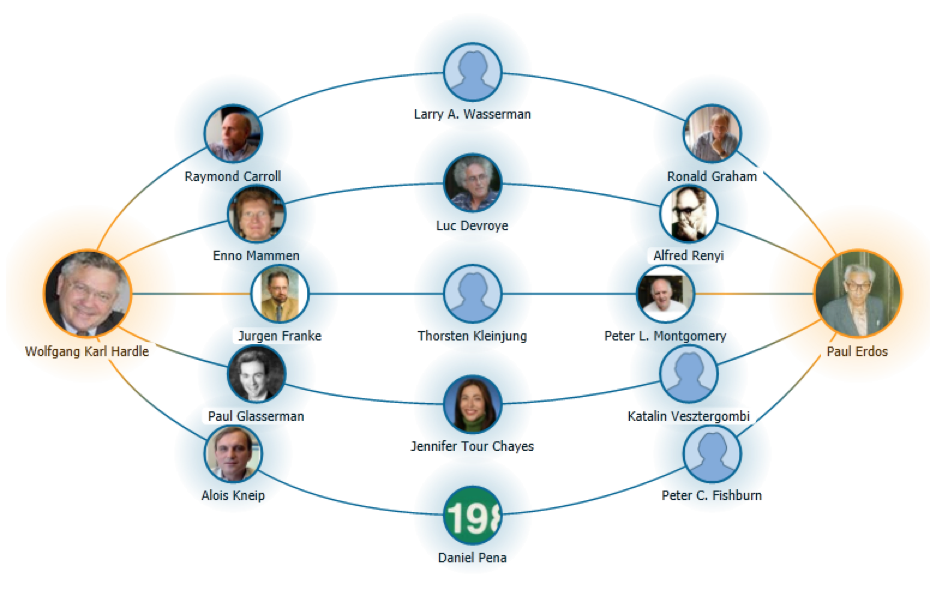
\includegraphics[scale=0.45]{figures/coauthorpath.png}
\caption{Coauthorship path of W.K. H\"ardle}
\bigskip
\scriptsize{
\href{http://academic.research.microsoft.com/VisualExplorer\#12530409\& 1112639}{Source: Microsoft Academic}}
\end{figure}
}

\frame{
\frametitle{A More Specific Coauthorship Graph}
\begin{figure}
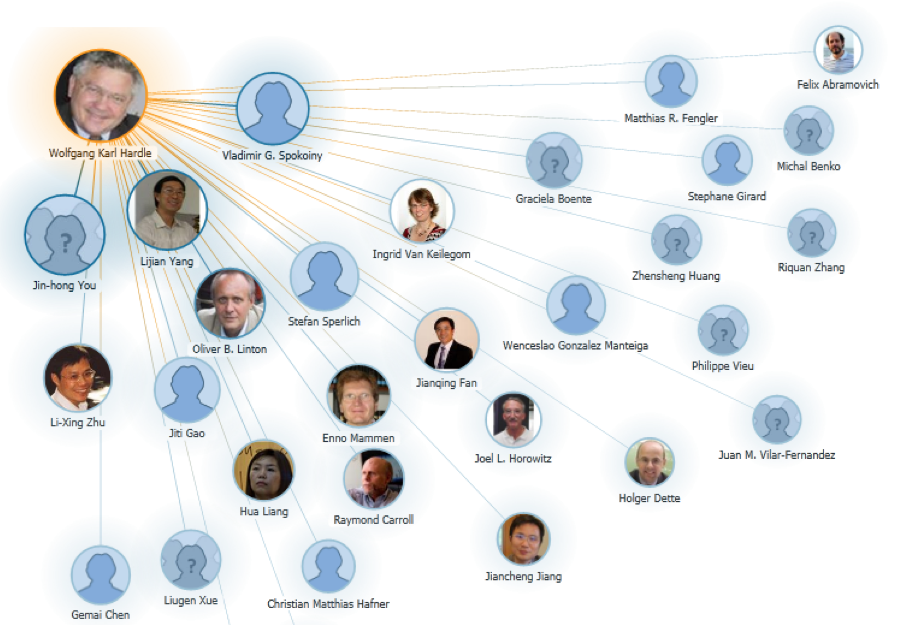
\includegraphics[scale=0.42]{figures/citationpath.png}
\caption{Citation path of W.K. H\"ardle}
\bigskip
\scriptsize{
\href{http://academic.research.microsoft.com/VisualExplorer\#12530409\& citation}{Source: Microsoft Academic}}
\end{figure}
}


\frame[plain]{
\frametitle{Outline}
\begin{enumerate}
\item Motivation \quad \checkmark
\item Definition
\item Relation to Adjacency Matrix
\item Node Centrality
\item Comparison of Various Node Centralities
\item Extension:Directed Cases
\item Graph Centrality
\item Examples of Various Graph Centralities 
\end{enumerate}
}

\section{Definition}
\frame{
\frametitle{Notation \& Terminology}
An \textbf{undirected graph} $\mathcal{G}=(\mathcal{V},\mathcal{E})$ consists of a list of vertices $\mathcal{V}=\{1,2,\ldots, N\}$ \,and a set of edges $\mathcal{E} = \{(i,j), (k,l), \ldots\}$ for $i, j, k, l \in \mathcal{V}$ where
\bigskip{}
\begin{itemize}
\item vertices $\mathcal{V}$: node, individual, agent,
\bigskip
\item edges $\mathcal{E}$: links, connections, ties.
\end{itemize}
}

\frame{
\frametitle{Notation \& Terminology}
A graph could be represented by its \textbf{adjacency matrix} $A = [a_{i,j}]$ where
\begin{displaymath}
 a_{i, j} = \left\{\begin{array}{ll} 
 1 & \textrm{if $(i, j) \in \mathcal{V}$}\\ 
 0 & otherwise \\  
 \end{array} \right. 
 \end{displaymath}
\begin{itemize}
\item $A$: symmetric binary matrix with diagonal to be zero.
\end{itemize}
}

\begin{frame}
\frametitle{Some Terms and Concepts of Graph Theory}
\text{A graph with five nodes and five edges:} 
\smallskip
\begin{columns}[onlytextwidth]
\hspace{-0.5 cm}
\begin{column}{0.5\textwidth}
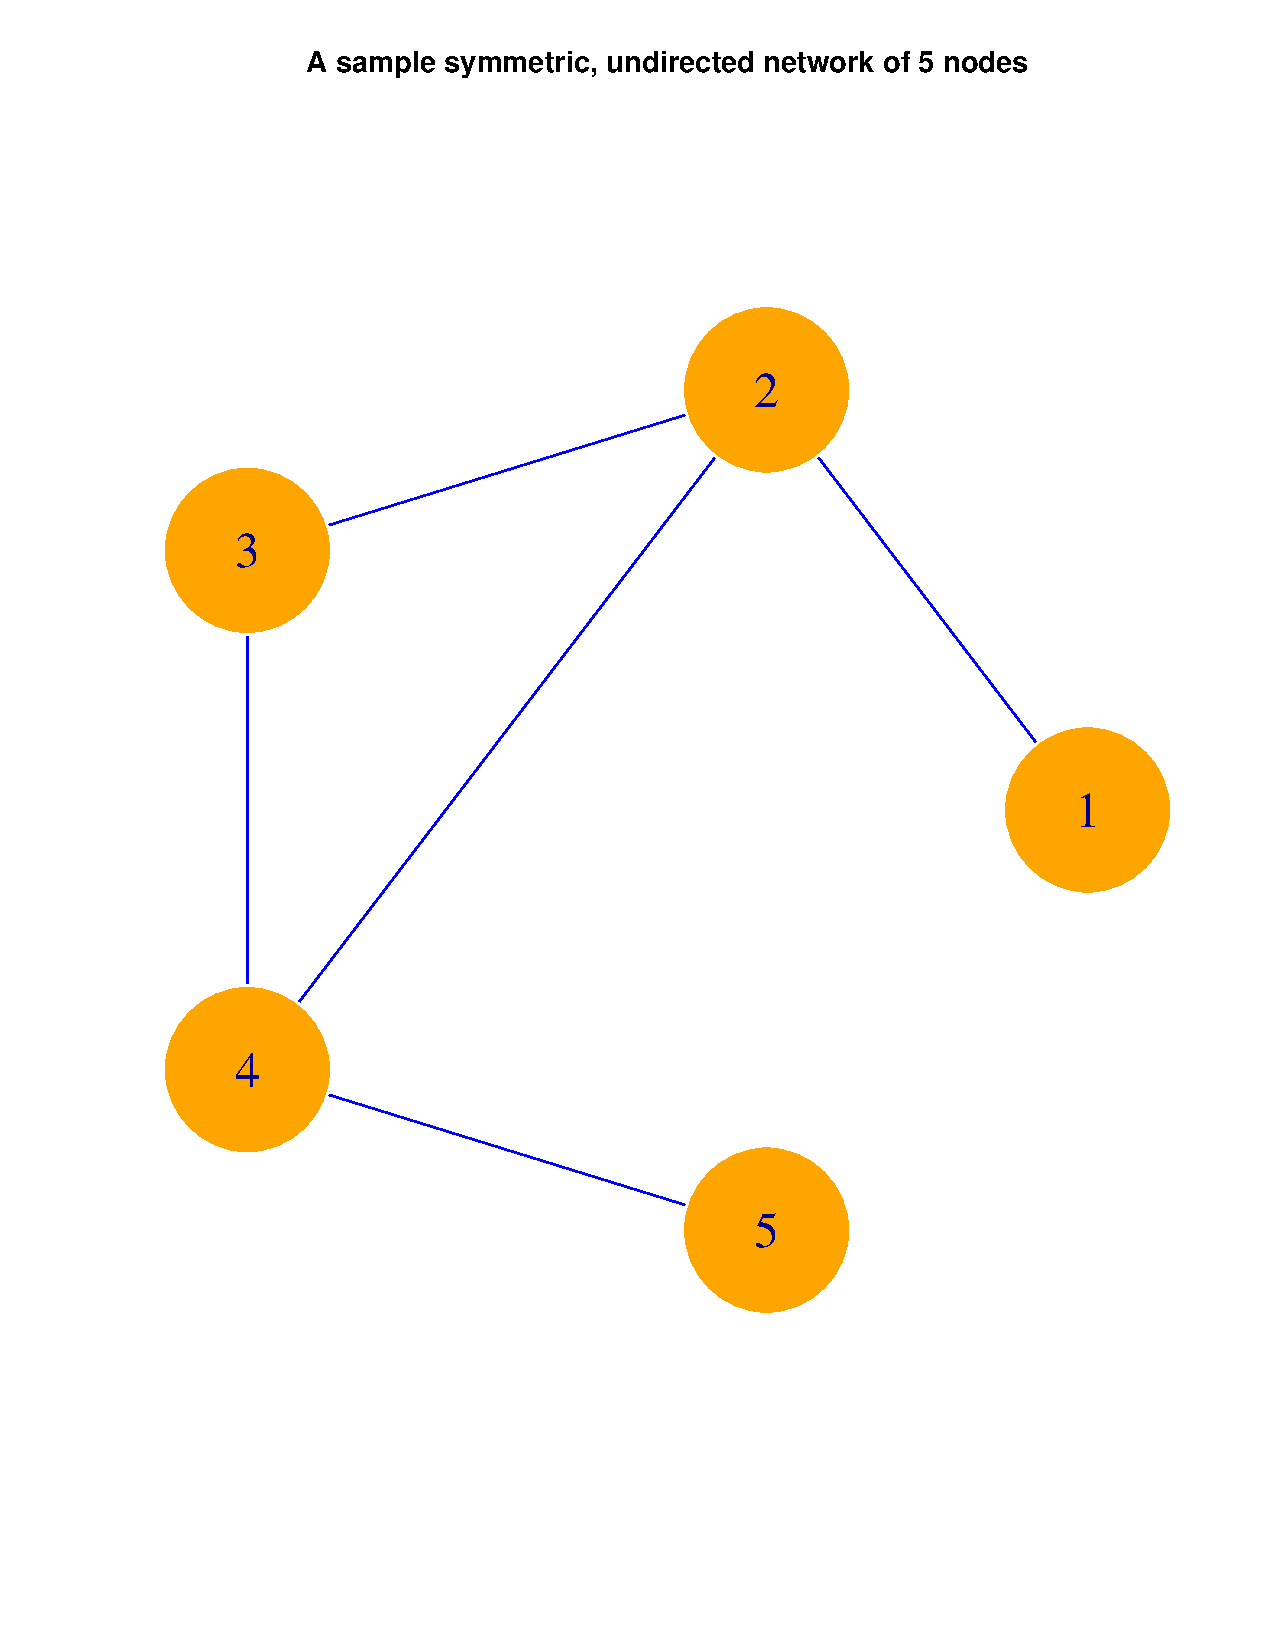
\includegraphics[scale=0.25]{picture1.pdf}
\end{column}
\hspace*{0.2cm}\begin{column}{0.5\textwidth}
\begin{itemize}
\begin{small}
\color{isegreen}
\item Degree: the number of other nodes to which a given node is adjacent,
\item Path: unordered pair of nodes, $(P_{i},P_{j})$ each is reachable,
\item Distance: the number of edges in that path,
\item Geodesics: the shortest paths linking a given pair of nodes.
\end{small}
\end{itemize}
\end{column}
\end{columns}
\end{frame}

\section{Adjacency Matrix}
\frame{
\frametitle{Adjacency Matrix \& Network}
\color{isegreen}
\textbf{Example 1:} symmetric, unweighted adjacency matrix with 4 nodes 
\smallskip
\begin{columns}[onlytextwidth]
\begin{column}{0.5\textwidth}

$
A =
  \begin{bmatrix}
    0 & 1 & 0 & 0 \\
    1 & 0 & 1 & 1 \\
    0 & 1 & 0 & 0 \\
    0 & 1 & 0 & 0 \\
  \end{bmatrix}
$
\end{column}
\color{black}
\hspace*{0.2cm}\begin{column}{0.5\textwidth}
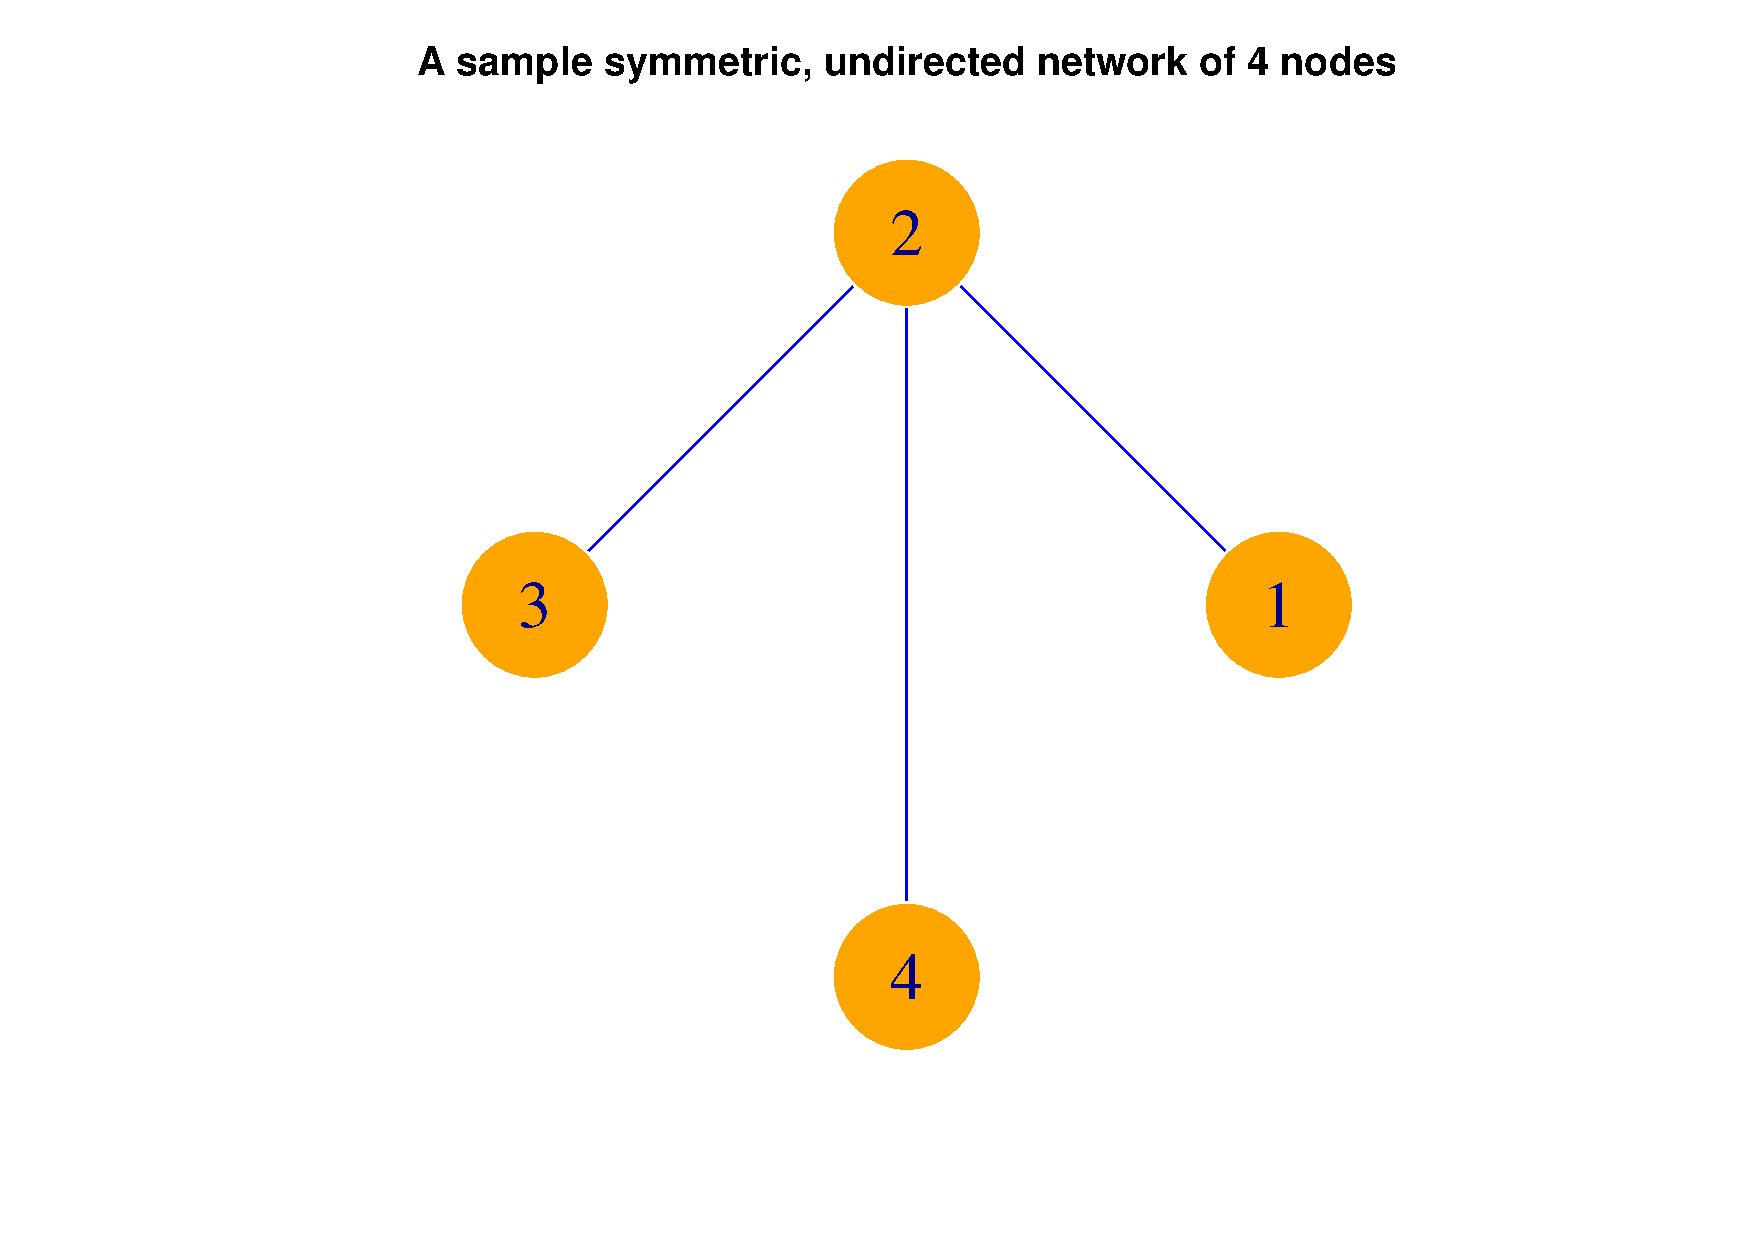
\includegraphics[scale=0.20]{figures/4nundirected.pdf}
\end{column}
\end{columns}
\href{https://github.com/QuantLet/METISNET/tree/master/METISNET-adjtonet}{\quantnet METISNET-adjtonet}
}


\frame{
\frametitle{Adjacency Matrix \& Network}
\color{isegreen}
\textbf{Example 2:} asymmetric, unweighted adjacency matrix with 4 nodes
\smallskip
\begin{columns}[onlytextwidth]
\begin{column}{0.5\textwidth}

$
A=
  \begin{bmatrix}
    0 & 0 & 1 & 0 \\
    0 & 0 & 1 & 0 \\
    0 & 1 & 0 & 0 \\
    1 & 0 & 1 & 0 \\
  \end{bmatrix}
$
\end{column}
\color{black}
\hspace*{0.2cm}\begin{column}{0.5\textwidth}
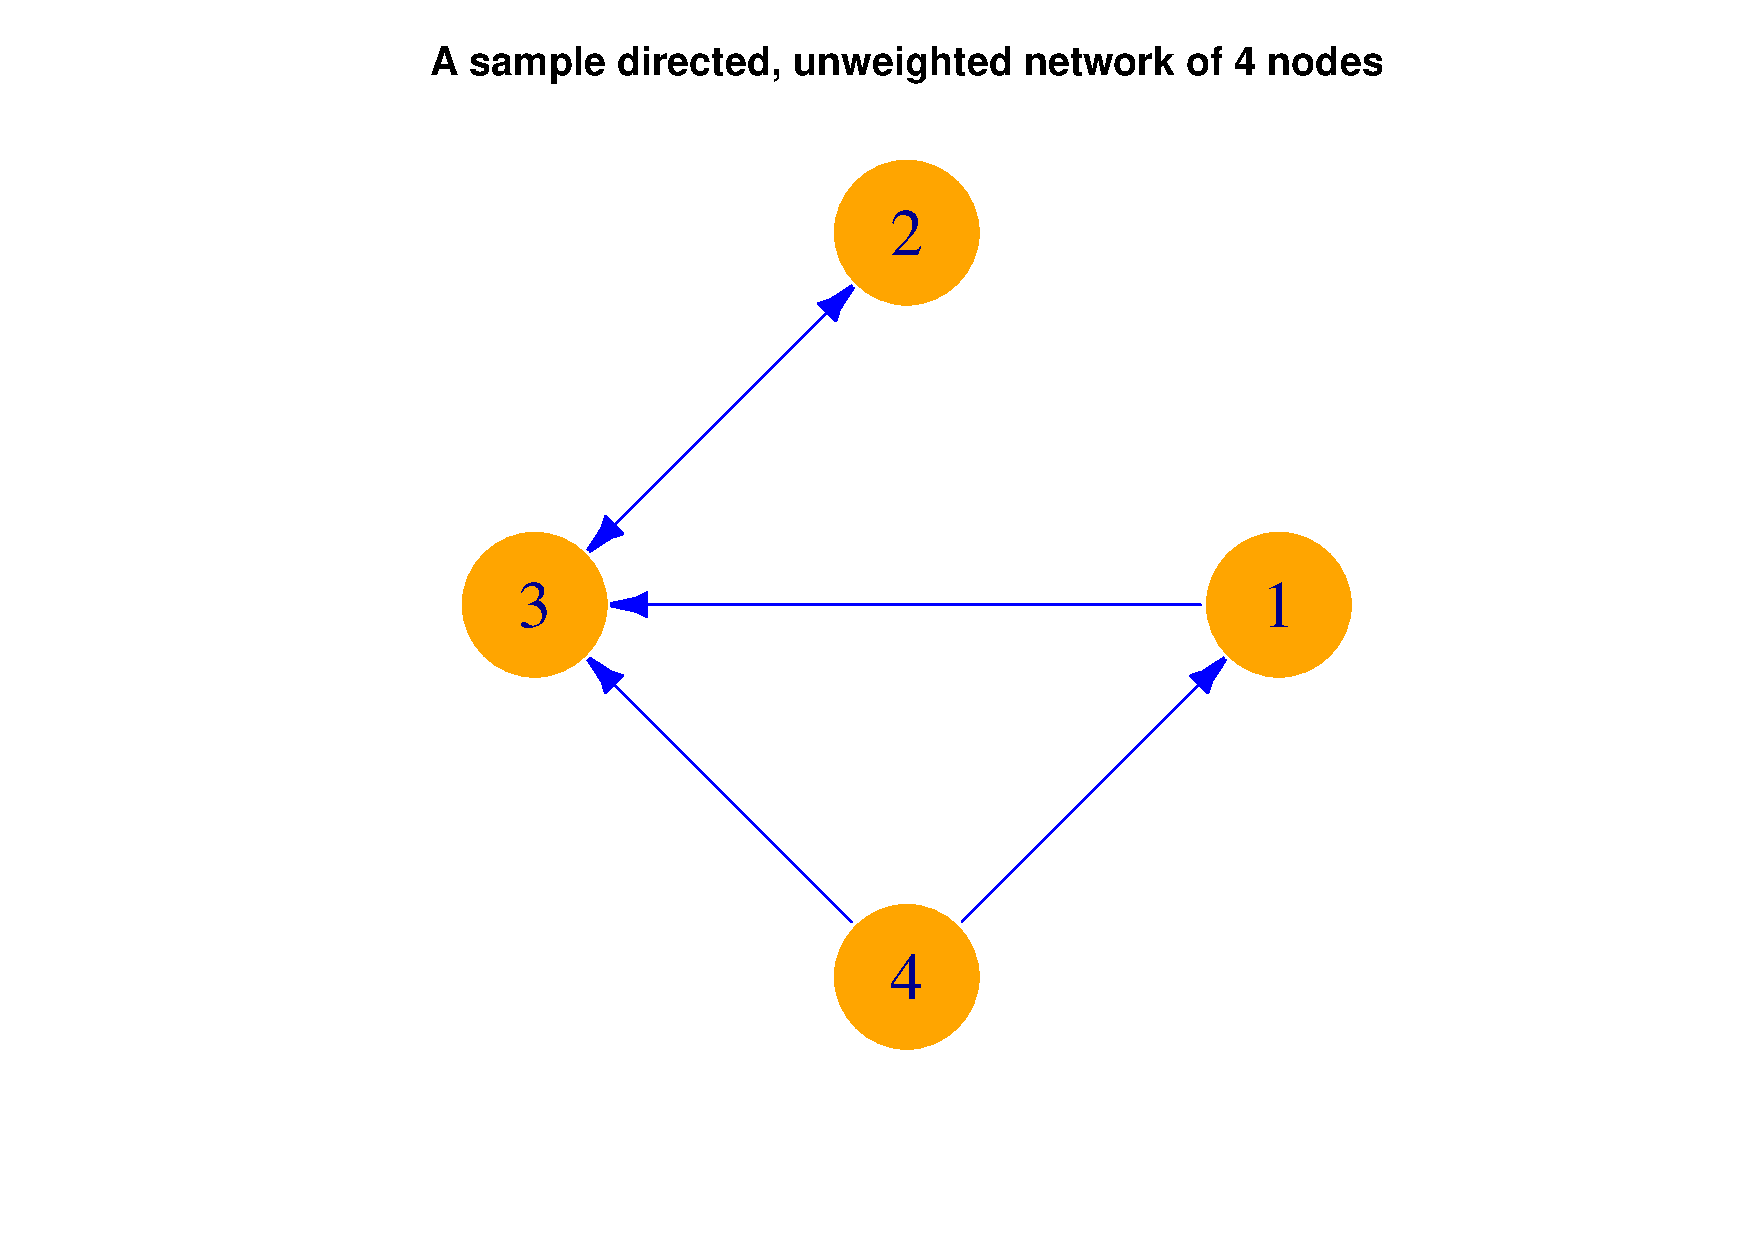
\includegraphics[scale=0.20]{figures/4ndirected.pdf}
\end{column}
\end{columns}
\href{https://github.com/QuantLet/METISNET/tree/master/METISNET-adjtonet}{\quantnet METISNET-adjtonet}
}


\frame{
\frametitle{Adjacency Matrix \& Network}
\color{isegreen}
\textbf{Example 3:} asymmetric, weighted adjacency matrix with 4 nodes
\smallskip
\begin{columns}[onlytextwidth]
\begin{column}{0.5\textwidth}

$
A=
  \begin{bmatrix}
    0 & 0.3 & 0.7 & 0 \\
    0 & 0 & 1 & 0 \\
    0 & 1 & 0 & 0 \\
    0.1 & 0 & 0.9 & 0 \\
  \end{bmatrix}
$
\end{column}
\color{black}
\hspace*{0.2cm}\begin{column}{0.5\textwidth}
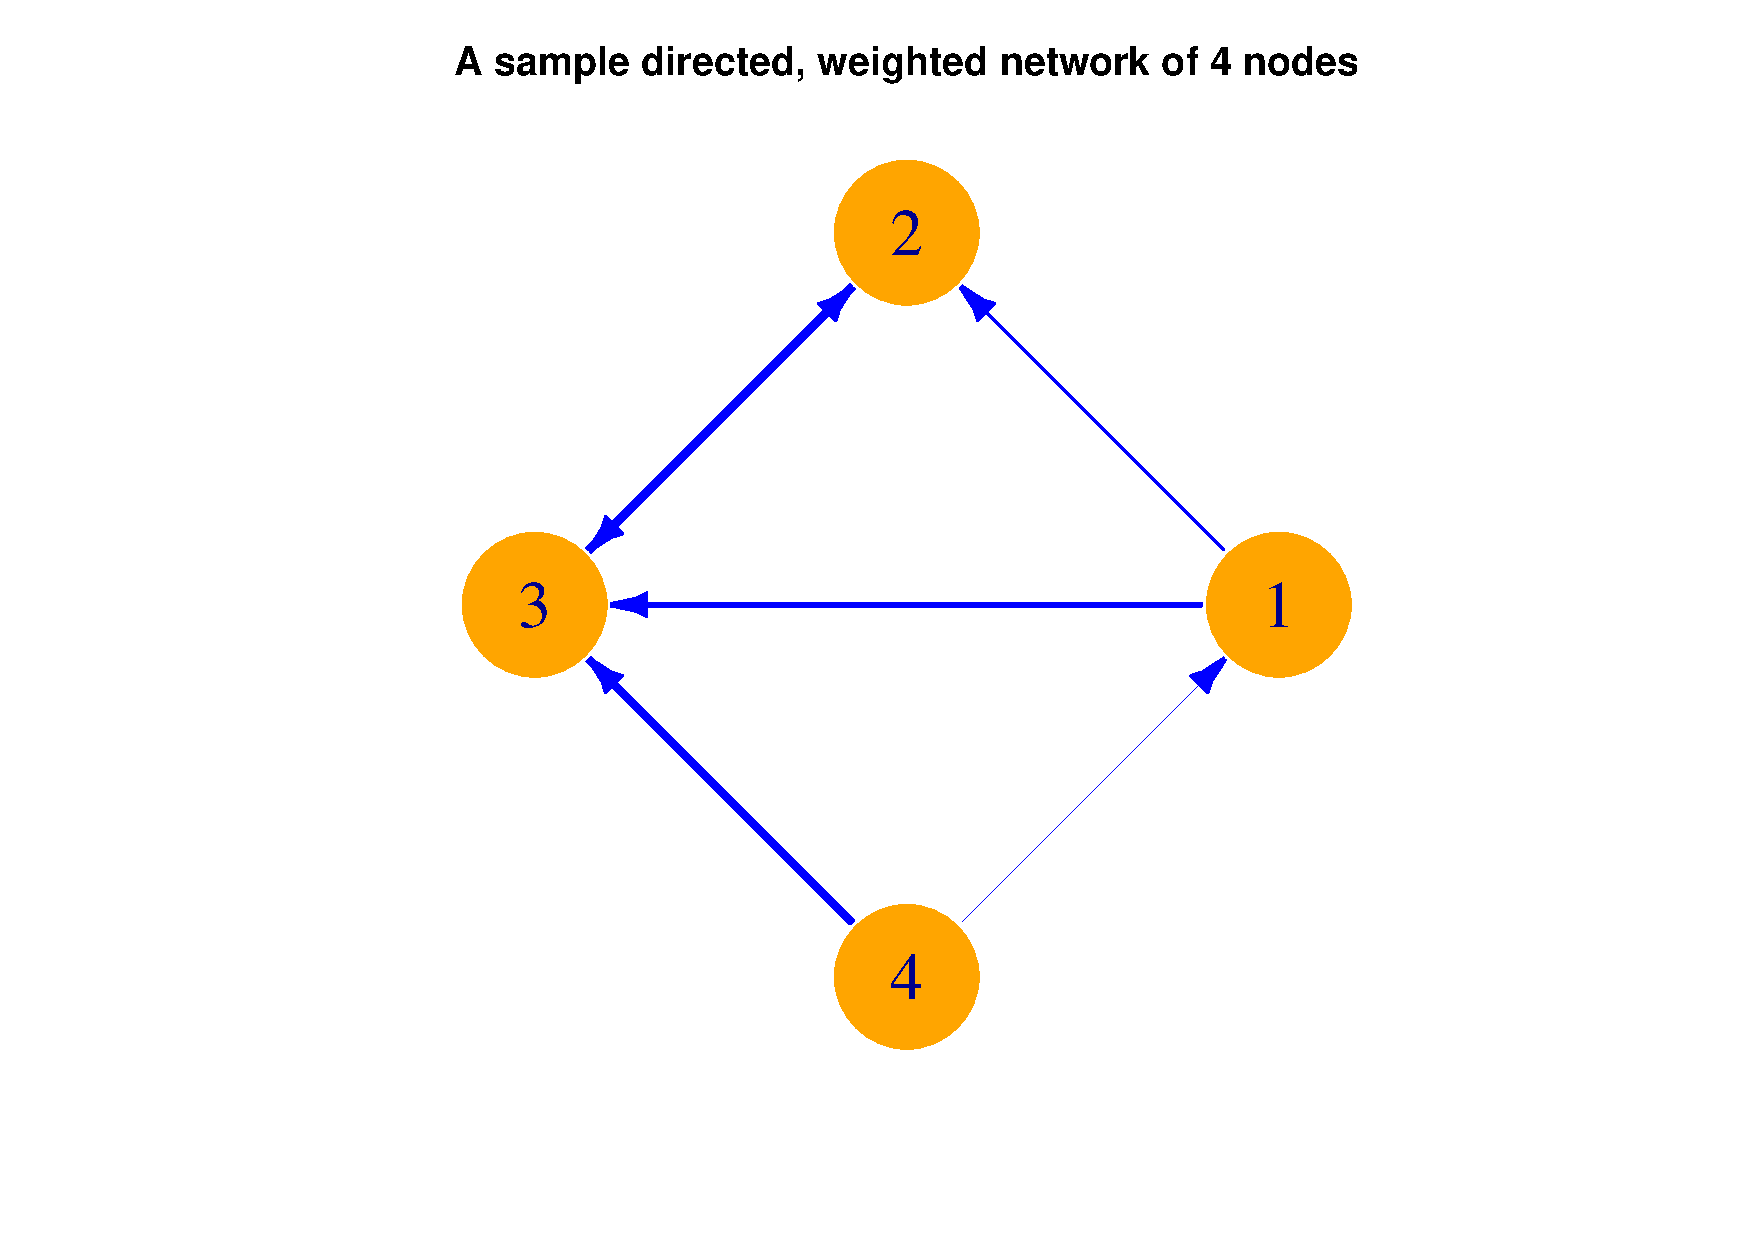
\includegraphics[scale=0.20]{figures/4ndirectedweighted.pdf}
\end{column}
\end{columns}
\href{https://github.com/QuantLet/METISNET/tree/master/METISNET-adjtonet}{\quantnet METISNET-adjtonet}
}

\section{Node Centrality}
%\subsection{Connectedness}
%\frame{
%\frametitle{Connectedness}
%\begin{itemize}
%\item To connectedness -- $C_{to}$
%\item From connectedness -- $C_{from}$
%\item Total connectedness -- $C_{total}$
%\end{itemize}
%}

%\frame{
%\frametitle{Connectedness}
%For an adjacency matrix $A = \{a_{ij}\}_{i,j=1}^n$ which denotes the network
%\begin{align*}
%C_{to,j} &= \sum_{i\neq j}a_{ij}, j = 1, 2, \ldots, n\\
%C_{from,j} &= \sum_{i\neq j}a_{ji},  j = 1, 2, \ldots, n\\
%C_{total} &= \frac{1}{n}\sum_{i,j=1}^{n}a_{ij}
%\end{align*} 
%}


\section{Node Centrality}
\begin{frame}
\frametitle{Three Distinct Structural Properties}
\begin{itemize}
	\item The position has the maximum possible degree,
	\item It falls on the geodesics between the largest possible number of other nodes, 
    \item It is maximally close to them.
\end{itemize}
\end{frame}

\subsection{Centrality}
\frame{\frametitle{Node Centrality}
\begin{itemize}
\item Degree centrality
\item Closeness centrality
\item Betweenness centrality
\item Eigenvector centrality
\item Katz centrality
\item PageRank centrality
\item Percolation centrality
\item Cross-clique centrality
\item Freeman Centrality
\end{itemize}
}
%%%%%%%%%%%%%%%%%%%%%%%%%%%%%%%%%%%%%%%%%%%%%%%%%%%
\begin{frame}
\frametitle{Degree Centrality}
Nieminen (1974) has introduced a simple, natural and perfectly general measure of centrality based upon degree.
For a network $\mathcal{G}=(\mathcal{V},\mathcal{E})$, degree centrality of a node $v_k$ equals
\color{iseblue}
\begin{displaymath}
C_{D}(v_{k})=\sum_{i=1}^n a(v_{i},v_{k})
\end{displaymath}
\color{black}
where 
\begin{displaymath}
 a(v_{i},v_{k}) = \left\{\begin{array}{ll}
1 & \textrm{if $v_{i}$ and $v_{k}$ are connected by a line,}\\
0 & \textrm{otherwise.}\\
\end{array} \right.
\end{displaymath}
\end{frame}

\begin{frame}
The magnitude of $C_{D}(v_{k})$ is partly a function of the size of the network on which it is calculated. To compare the relative
centrality of nodes from different graphs, for example, we need a measure from which the effect of network size has been removed.	
\\
\bigskip
A given node, $v_{k}$ can at most be adjacent to $n-1$ other nodes in a graph. The maximum of $C_{D}(v_{k})$, therefore, is $n-1$. Then
\color{iseblue}
\begin{displaymath}
C'_{D}(v_{k})=\frac{\sum_{i=1}^n a(v_{i},v_{k})}{n-1}
\end{displaymath}
\end{frame}

\begin{frame}
\textbf{Assumptions}
\begin{itemize}
\item a measure of immediate effects(t+1) only
\item models the frequency of visits by something taking an infinitely long random walk through a network
\end{itemize}
\bigskip
\textbf{Applicable processes}
\begin{itemize}
\item parallel duplication flow processes
\item walk-based transfer processes such as the money exchange process
\end{itemize}
\end{frame}

%%%%%%%%%%%%%%%%%%%%%%%%%%%%%%%%%%%%%%%%%%%%%%%%%%
\begin{frame}
\frametitle{Closeness Centrality}
Closeness-based measures of node centrality have been developed by Bavelas (1950), Beauchamp (1965), Sabidussi (1966), Moxley (1974) and Rogers (1974). The simplest and most natural of these measures is Sabidussi's (1966). 
For a network $\mathcal{G}=(\mathcal{V},\mathcal{E})$, closeness centrality equals
\color{iseblue}
\begin{equation}
	C_C(v_k) = \frac{1}{\sum_{i=1}^n d(v_i, v_k)}
\end{equation}
\color{black}
\begin{itemize}
\item $d(v_i, v_k)$: the number of edges in the geodesic linking $v_i$ and $v_k$
\end{itemize}
\end{frame}

\begin{frame}
Beauchamp (1965) derived the relative centrality based on closeness measure.
\color{iseblue}
\begin{equation}
	C_C'(v_k) = \frac{n-1}{\sum_{i=1}^n d(v_i, v_k)}
\end{equation}
\end{frame}

\frame{
\textbf{Assumptions}
\begin{itemize}
\item flow along shortest paths or flow by parallel duplication \\
\item shortest path assumptions: only works on connected graphs;\\ taking shortest paths implies taking valid paths
\end{itemize}
\bigskip
\textbf{Applicable processes}
\begin{itemize}
\item geodesic paths
\item parallel duplication flow processes
\end{itemize}
}

%%%%%%%%%%%%%%%%%%%%%%%%%%%%%%%%%%%%%%%%%%%%%%%%%%
\begin{frame}
\frametitle{Betweenness Centrality}
Shaw (1954) included betweenness counts in a complex empirically based measure of centrality, but he did not develop a measure of betweenness. Direct measures were developed independently by Anthonisse (1971) and Freeman (1977).	For a network $\mathcal{G}=(\mathcal{V},\mathcal{E})$, betweenness centrality equals
\color{iseblue}
\begin{displaymath}
C_{B}(v_{k})=\sum_{i<j}^n\sum_{j}^n \frac {g_{ij}(v_{k})}{g_{ij}}
\end{displaymath}
\color{black}
\begin{itemize}
\item $g_{ij}$: the number of geodesics linking $v_{i}$ and $v_{j}$
\item $g_{ij}(v_{k})$: the number of geodesics linking $v_{i}$ and $v_{j}$ that contain $v_{k}$
\end{itemize}
\end{frame}

\begin{frame}
Freeman (1977) proved that the maximum value taken by $C_{B}(v_{k})$ is achieved only by the central node in a star. It is $\frac {n^2-3n+2}{2}$.
\\
\bigskip
Therefore, the relative centrality of any node in a graph may be expressed as a ratio,
\color{iseblue}
\begin{displaymath}
C'_{B}(v_{k})=\frac{2C_{B}(v_{k})}{n^2-3n+2}
\end{displaymath}
\end{frame}

\frame{
\textbf{Assumptions}
\begin{itemize}
\item the traffic is indivisible(transfer)
\item the traffic travels only along shortest paths
\end{itemize}
\bigskip
\textbf{Applicable processes}
\begin{itemize}
\item package delivery process
\end{itemize}
}


\frame{
\frametitle{More about 'distance'}
\begin{itemize}
\item related to $C_{C}$ and $C_{B}$
\item the number of edges in the shortest connecting path (in the sense of edge number) -- unweighted
\item the real length of shortest connecting path (in the sense of real length)-- weighted
\item considered as a 'cost'
\end{itemize}
Example is given at the end of this talk : Minnesota Road Networks
}
 


\frame{
\frametitle{Eigenvector Centrality}
For a network $\mathcal{G}=(\mathcal{V},\mathcal{E})$, eigenvector centrality equals
\color{iseblue}
\begin{align*}
C_{E}(v) &=\frac{1}{\lambda}\sum_{t \in M(v)} C_{E}(t) = \frac{1}{\lambda} \sum_{t \in \mathcal{G}}a_{v,t} C_{E}(t)\\
\lambda C_{E} &= AC_{E}
\end{align*}
\color{black}
\begin{itemize}
\item $A=\{a_{v,t}\}_{v,t=1}^N$ is a 0-1 adjacency matrix
\item $\lambda$: maximum eigenvalue of $A$
\item $M(v)$: set of neighbors of $v$
\item $a_{v,t}$: the $vt_{th}$ element of $A$
\end{itemize}
}

\frame{
\bigskip
\textbf{Assumptions}
\begin{itemize}
\item the traffic is able to move via unrestricted walks\\
\item each node affects all of its neighbors simultaneously
\end{itemize}
\bigskip
\textbf{Applicable processes}
\begin{itemize}
\item influence type processes
\end{itemize}
}


\section{Comparison of Various Node Centralities}
\frame{
\frametitle{which is the central node?}
\color{isegreen}
\textbf{Example 4:} 
\smallskip
\begin{columns}[onlytextwidth]
\hspace{-2cm}
\begin{column}{0.5\textwidth}
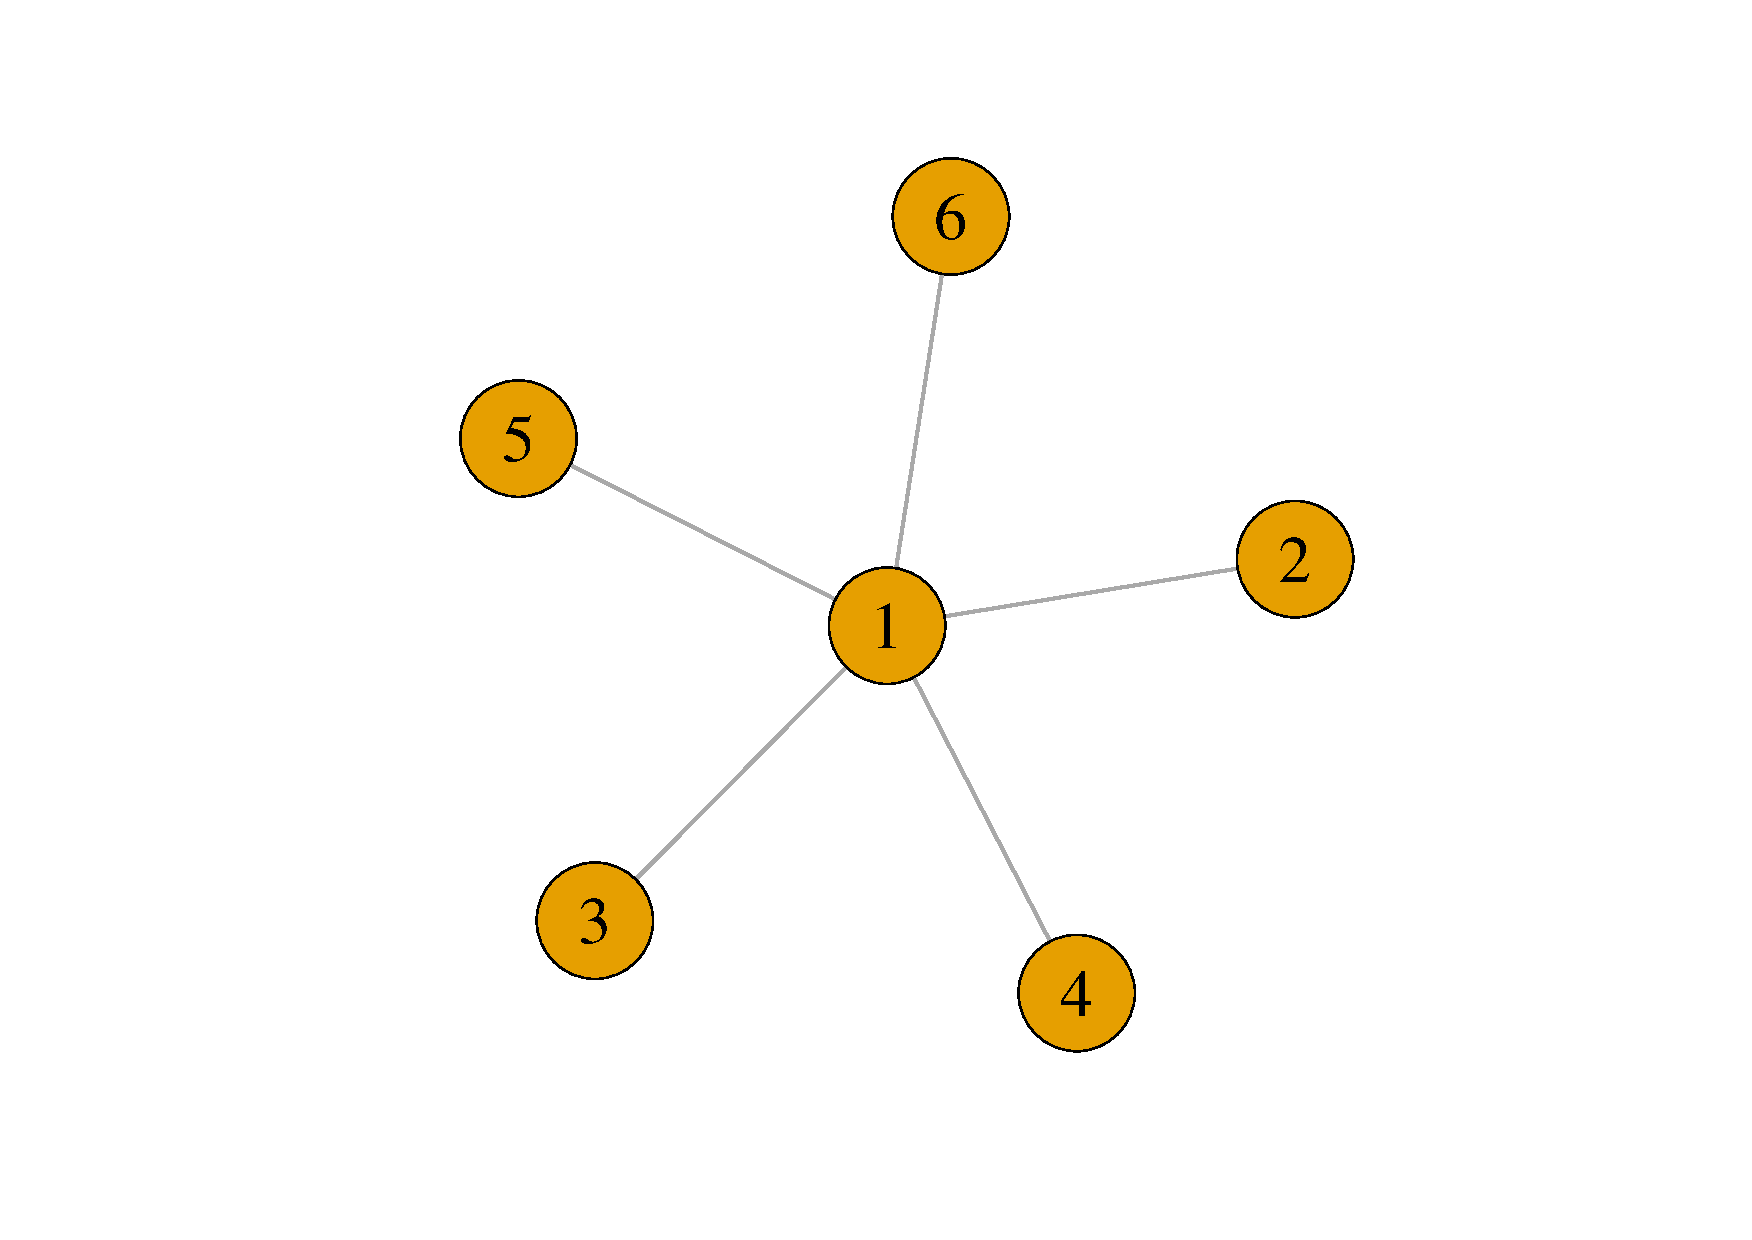
\includegraphics[scale=0.30]{figures/star.pdf}
\end{column}

\hspace*{0.2cm}\begin{column}{0.5\textwidth}
\begin{itemize}
\begin{small}
\color{isegreen}
\item $\mathbf{C_{D}(1) = 5}, C_{D}(2) = C_{D}(3) = C_{D}(4) = C_{D}(5) = C_{D}(6) = 1$
\item $\mathbf{C_{C}(1) = 1}, C_{C}(2) = C_{C}(3) = C_{C}(4) = C_{C}(5) = C_{C}(6) = 0.56$
\item $\mathbf{C_{B}(1) = 1}, C_{B}(2) = C_{B}(3) = C_{B}(4) = C_{B}(5) = C_{B}(6) = 0$
\item $\mathbf{C_{E}(1) = 0.71}, C_{E}(2) = C_{E}(3) = C_{E}(4) = C_{E}(5) = C_{E}(6) = 0.32$
\end{small}
\end{itemize}
\end{column}
\end{columns}
\color{black}
\vspace{-0.5cm}
\href{https://github.com/QuantLet/METISNET/tree/master/METISNET-adjtonet}{\quantnet METISNET-centralitymeasures}
}

%\frame{
%\frametitle{which is the central node?}
%\color{isegreen}
%\textbf{Example:} 
%\smallskip
%\begin{columns}[onlytextwidth]
%\begin{column}{0.5\textwidth}
%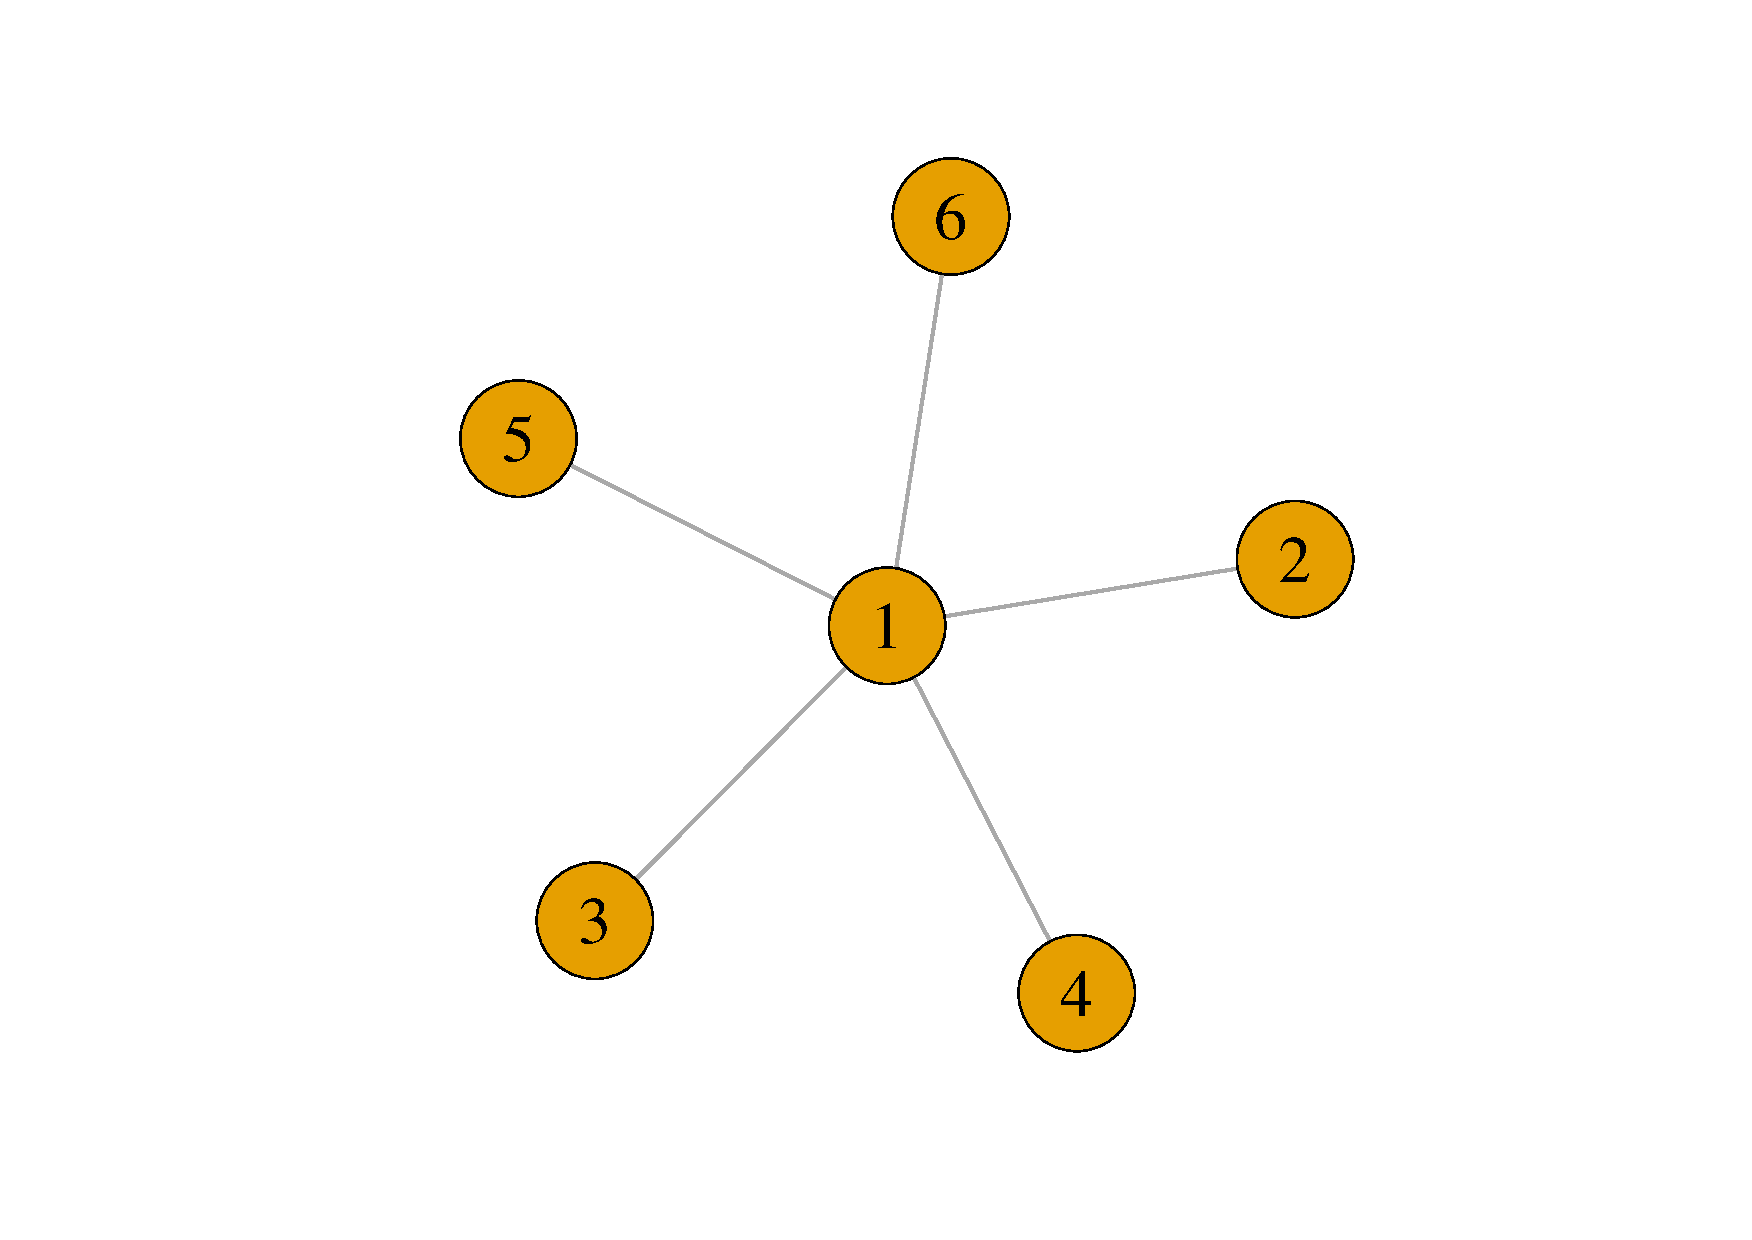
\includegraphics[scale=0.20]{figures/star.pdf}
%\end{column}
%\hspace*{0.2cm}\begin{column}{0.5\textwidth}
%\begin{itemize}
%\begin{tiny}
%\color{isegreen}
%\item degree centrality: node 1 has centrality 5, all others have centrality 1;
%\item closeness centrality: node 1 has centrality 1, all others have centrality 0.56;
%\item betweenness centrality: node 1 has centrality 1, all others have centrality 0;
%\item eigenvector centrality: node 1 has centrality 0.71, all others have centrality 0.32;
%\end{tiny}
%\end{itemize}
%\end{column}
%\end{columns}
%Conclusion: Node 1 is the central node by all centrality measures
%}

\frame{
\frametitle{which is the central node?}
\color{isegreen}
\textbf{Example 5:} 
\smallskip
\begin{columns}[onlytextwidth]
\hspace{-2cm}
\begin{column}{0.5\textwidth}
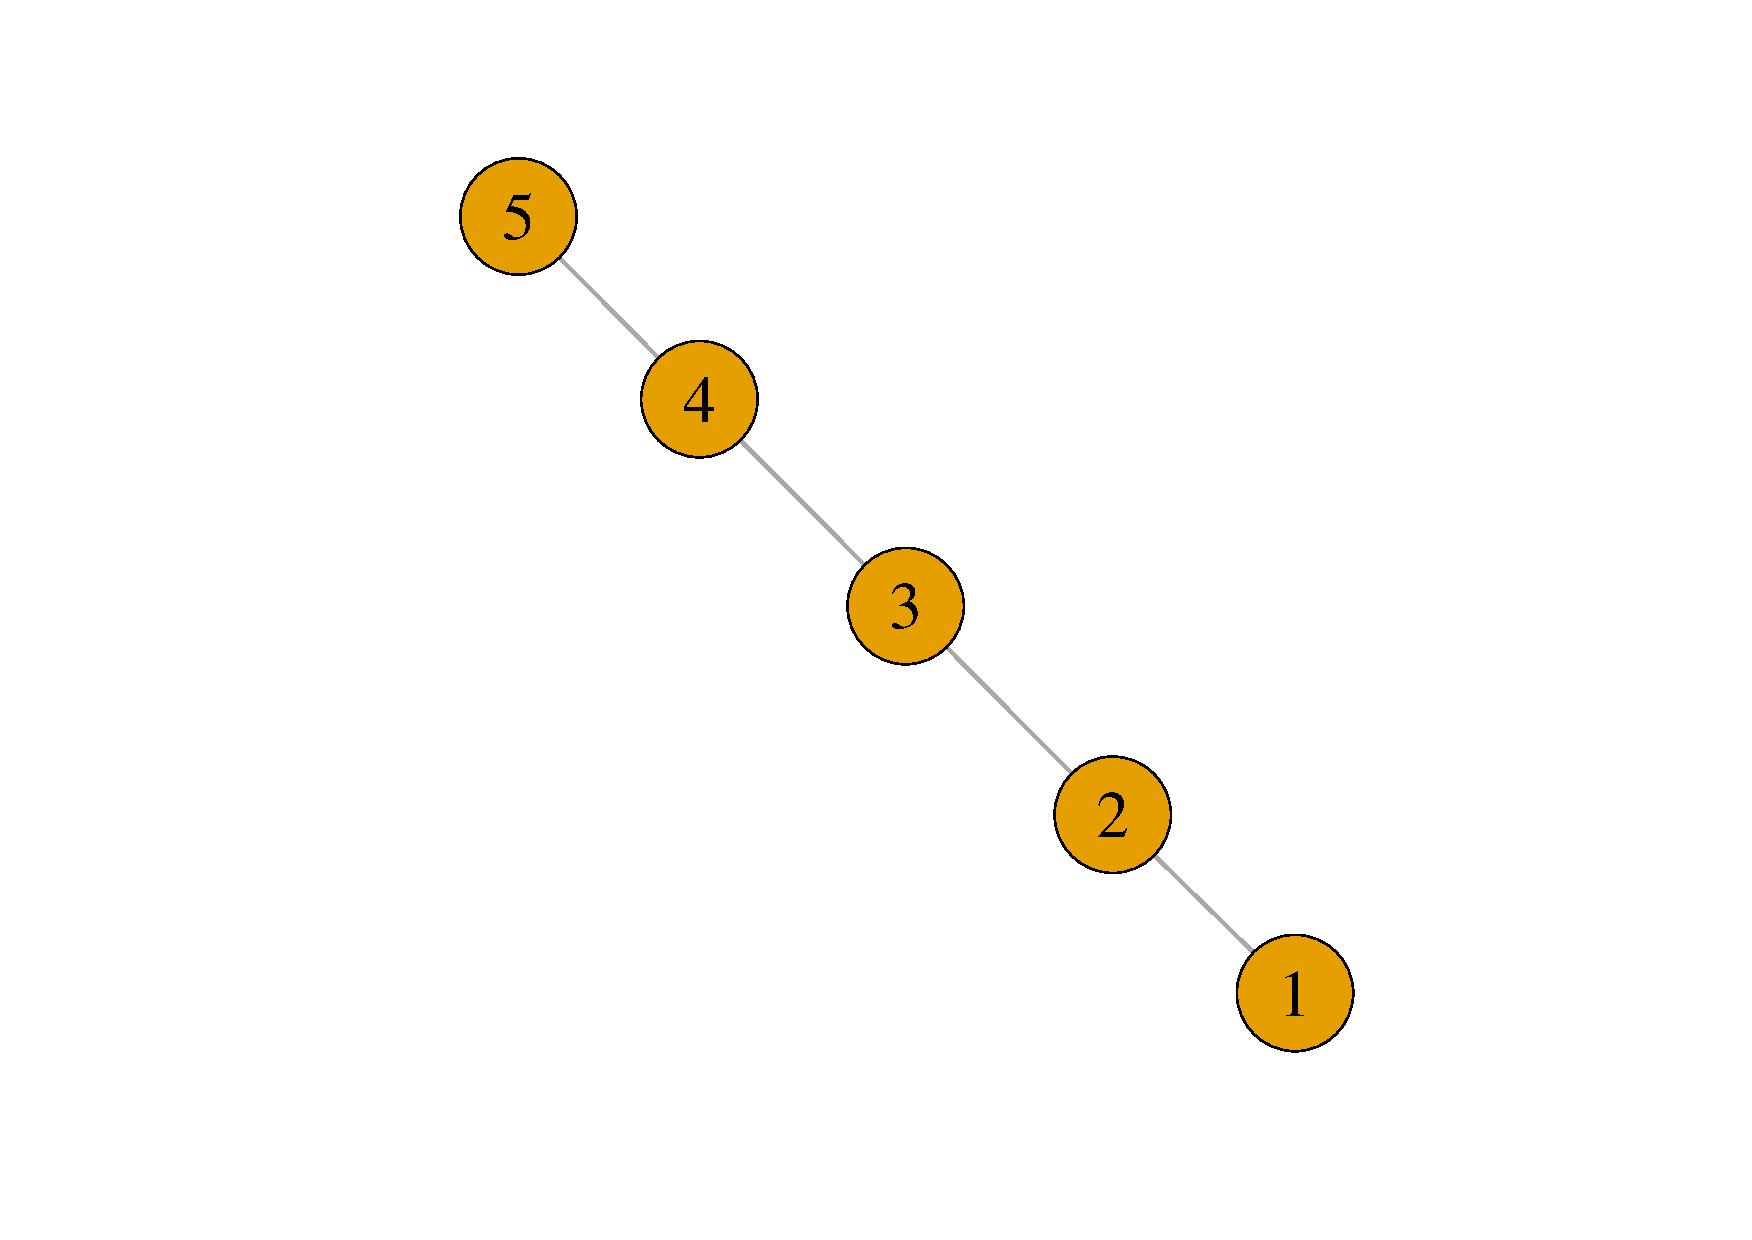
\includegraphics[scale=0.3]{figures/line.pdf}
\end{column}
\hspace*{0.2cm}\begin{column}{0.5\textwidth}
\begin{itemize}
\begin{small}
\color{isegreen}
\item $C_{D}(1) = C_{D}(5) = 1, \mathbf{C_{D}(2) = C_{D}(3) = C_{D}(4) = 2}$
\item $C_{C}(1) = C_{C}(5) = 0.4, C_{C}(2) = C_{C}(4) = 0.57, \mathbf{C_{C}(3) = 0.67}$
\item $C_{B}(1) = C_{B}(5) = 0, C_{B}(2) = C_{B}(4) = 0.50, \mathbf{C_{B}(3) = 0.67}$
\item $C_{E}(1) = C_{E}(5) = 0.29, C_{E}(2) = C_{E}(4) = 0.50, \mathbf{C_{B}(3) = 0.58}$
\end{small}
\end{itemize}
\end{column}
\end{columns}
\color{black}
\vspace{-0.8cm}
\href{https://github.com/QuantLet/METISNET/tree/master/METISNET-adjtonet}{\quantnet METISNET-centralitymeasures}
}

%\frame{
%\frametitle{which is the central node?}
%\color{isegreen}
%\textbf{Example:} 
%\smallskip
%\begin{columns}[onlytextwidth]
%\begin{column}{0.5\textwidth}
%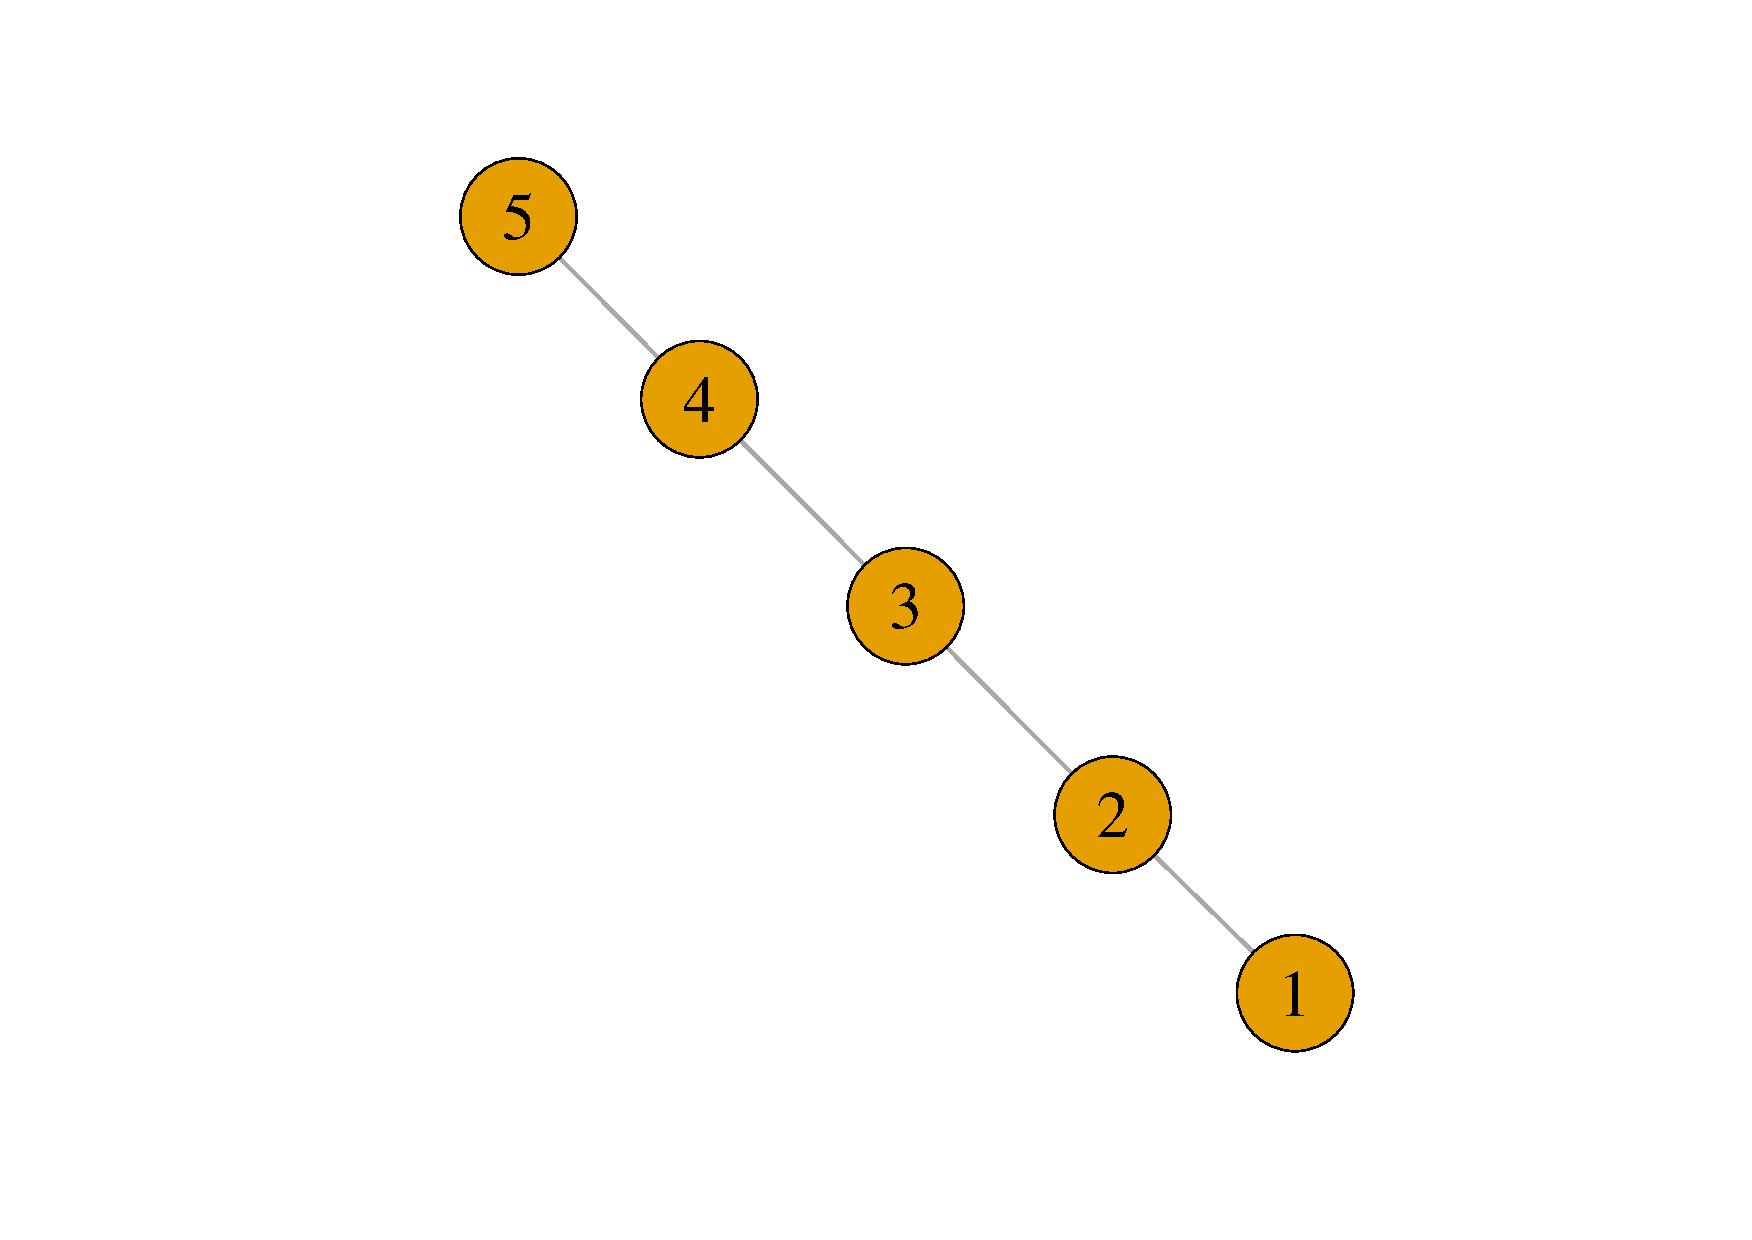
\includegraphics[scale=0.20]{figures/line.pdf}
%\end{column}
%\hspace*{0.2cm}\begin{column}{0.5\textwidth}
%\begin{itemize}
%\begin{tiny}
%\color{isegreen}
%\item degree centrality: node 1 and node 5 have centrality 1, all others have centrality 2;
%\item closeness centrality: node 1 and node 5 have centrality 0.4, node 2 and node 4 have centrality 0.57, node 3 has centrality 0.67;
%\item betweenness centrality: node 1 and node 5 have centrality 0, node 2 and node 4 have centrality 0.50, node 3 has centrality 0.67;
%\item eigenvector centrality: node 1 and node 5 have centrality 0.29, node 2 and node 4 have centrality 0.50, node 3 has centrality 0.58;
%\end{tiny}
%\end{itemize}
%\end{column}
%\end{columns}
%Conclusion: Node 3 is the central node by all centrality measures
%}

\frame{
\frametitle{which is the central node?}
\color{isegreen}
\textbf{Example 6:} 
\smallskip
\begin{columns}[onlytextwidth]
\hspace{-2cm}
\begin{column}{0.5\textwidth}
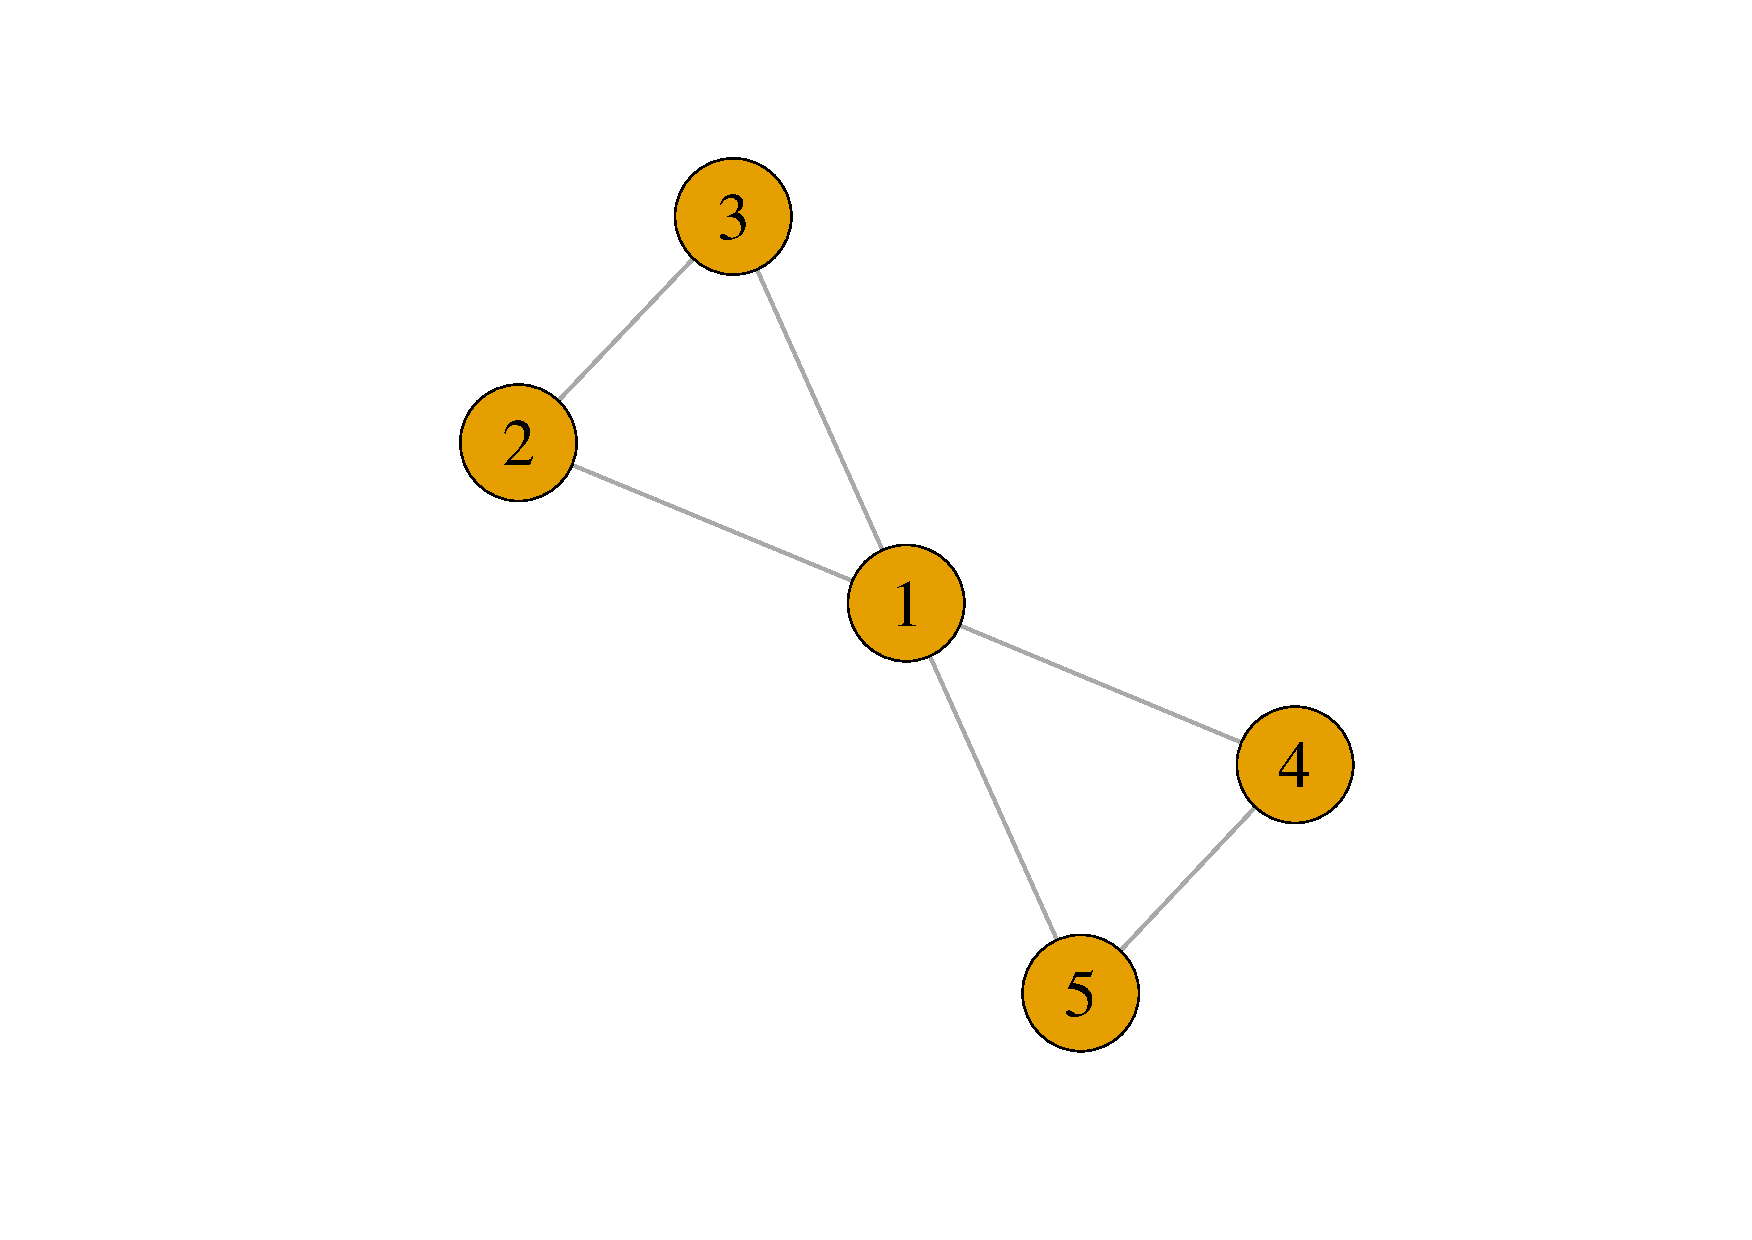
\includegraphics[scale=0.3]{figures/fork.pdf}
\end{column}
\hspace*{0.2cm}\begin{column}{0.5\textwidth}
\begin{itemize}
\begin{small}
\color{isegreen}
\item $\mathbf{C_{D}(1) = 4}, C_{D}(2) = C_{D}(3) = C_{D}(4) = C_{D}(5)= 2$
\item $\mathbf{C_{C}(1) = 1}, C_{C}(2) = C_{C}(3) = C_{C}(4) = C_{C}(5)= 0.67$
\item $\mathbf{C_{B}(1) = 0.67}, C_{B}(2) = C_{B}(3) = C_{B}(4) = C_{B}(5)= 0$
\item $\mathbf{C_{E}(1) = 0.62}, C_{E}(2) = C_{E}(3) = C_{E}(4) = C_{E}(5)= 0.39$
\end{small}
\end{itemize}
\end{column}
\end{columns}
\color{black}
\vspace{-0.8cm}
\href{https://github.com/QuantLet/METISNET/tree/master/METISNET-adjtonet}{\quantnet METISNET-centralitymeasures}
}

%\frame{
%\frametitle{which is the central node?}
%\color{isegreen}
%\textbf{Example:} 
%\smallskip
%\begin{columns}[onlytextwidth]
%\begin{column}{0.5\textwidth}
%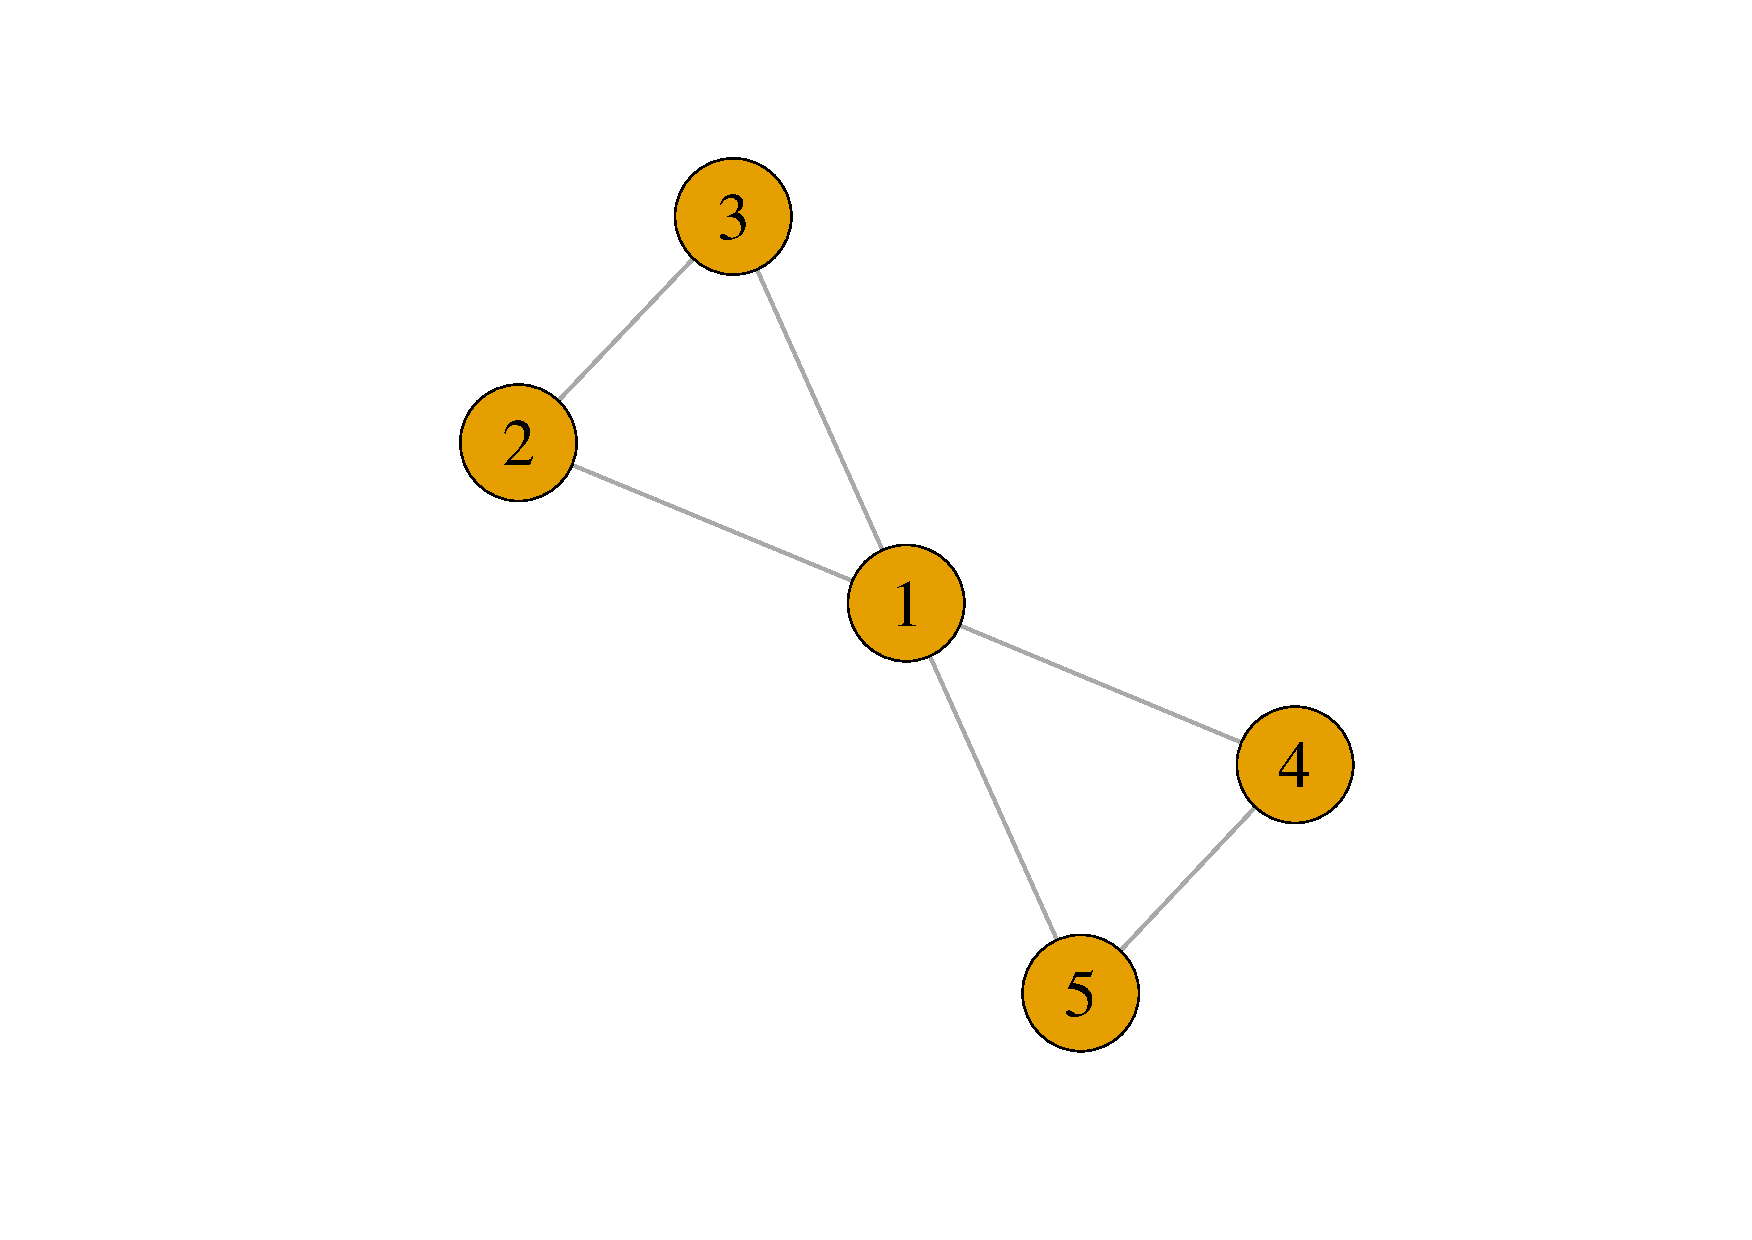
\includegraphics[scale=0.20]{figures/fork.pdf}
%\end{column}
%\hspace*{0.2cm}\begin{column}{0.5\textwidth}
%\begin{itemize}
%\begin{tiny}
%\color{isegreen}
%\item degree centrality: node 1 has centrality 4, all others have centrality 2;
%\item closeness centrality: node 1 has centrality 1, all others have centrality 0.67;
%\item betweenness centrality: node 1 has centrality 0.67, all others have centrality 0;
%\item eigenvector centrality: node 1 has centrality 0.62, all others have centrality 0.39;
%\end{tiny}
%\end{itemize}
%\end{column}
%\end{columns}
%Conclusion: Node 1 is the central node by all centrality measures
%}

\frame{
\frametitle{which is the central node?}
\color{isegreen}
\textbf{Example 7:}
\smallskip
\begin{columns}[onlytextwidth]
\hspace{-2cm}
\begin{column}{0.5\textwidth}
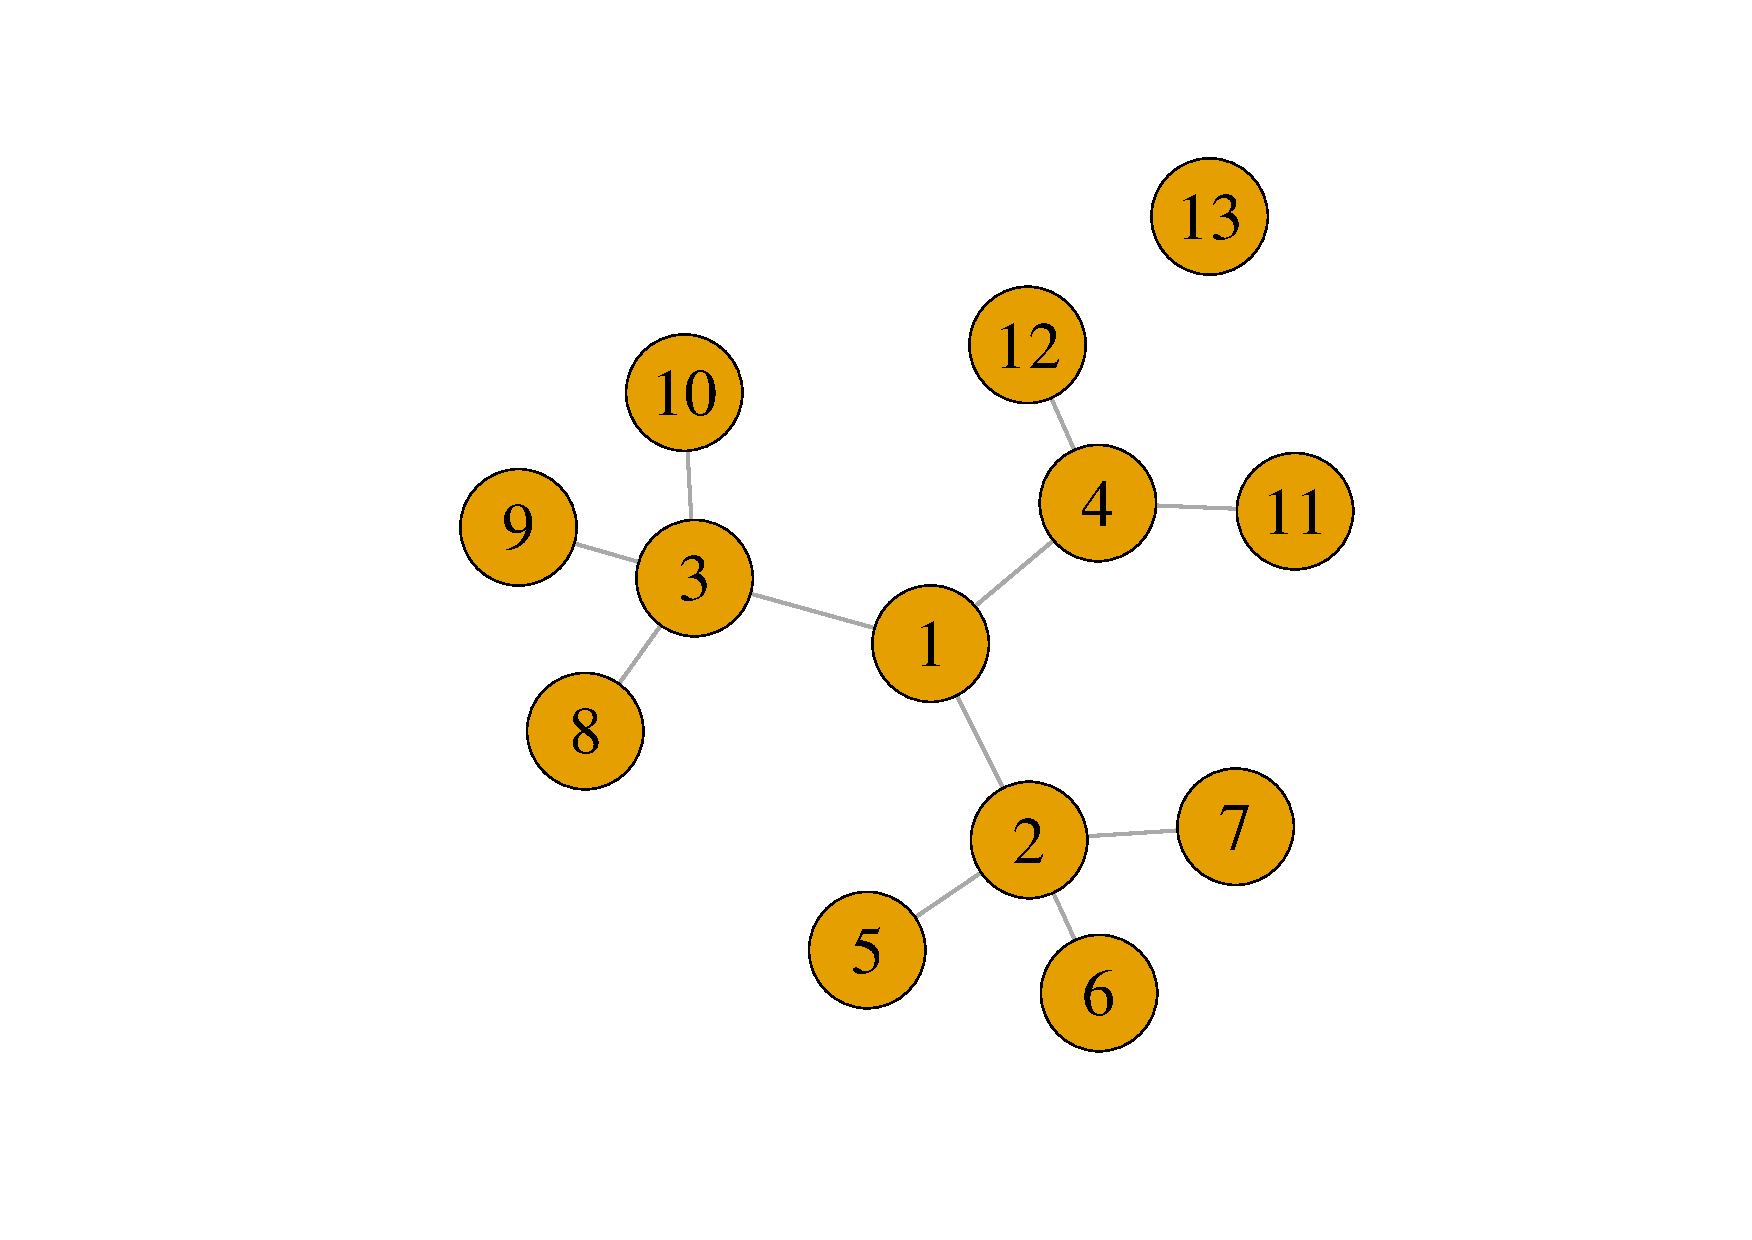
\includegraphics[scale=0.3]{figures/conteg.pdf}
\end{column}
\hspace*{0.2cm}\begin{column}{0.5\textwidth}
\begin{itemize}
\begin{small}
\color{isegreen}
\item $C_{D}(1) = C_{D}(4) = 3, \mathbf{C_{D}(2) = C_{D}(3) = 4}$
\item $\mathbf{C_{C}(1) = 0.63}, C_{C}(2) = C_{C}(3) = 0.52, C_{C}(4) = 0.48$
\item $\mathbf{C_{B}(1) = 0.61}, C_{B}(2) = C_{B}(3) = 0.36, C_{B}(4) = 0.27$
\item $\mathbf{C_{E}(1) = 0.51}, C_{E}(2) = C_{E}(3) = 0.44, C_{E}(4) = 0.33$
\end{small}
\end{itemize}
\end{column}
\end{columns}
\color{black}
\vspace{-1cm}
\href{https://github.com/QuantLet/METISNET/tree/master/METISNET-adjtonet}{\quantnet METISNET-centralitymeasures}
}

%\frame{
%\frametitle{which is the central node?}
%\color{isegreen}
%\textbf{Example:}
%\smallskip
%\begin{columns}[onlytextwidth]
%\begin{column}{0.5\textwidth}
%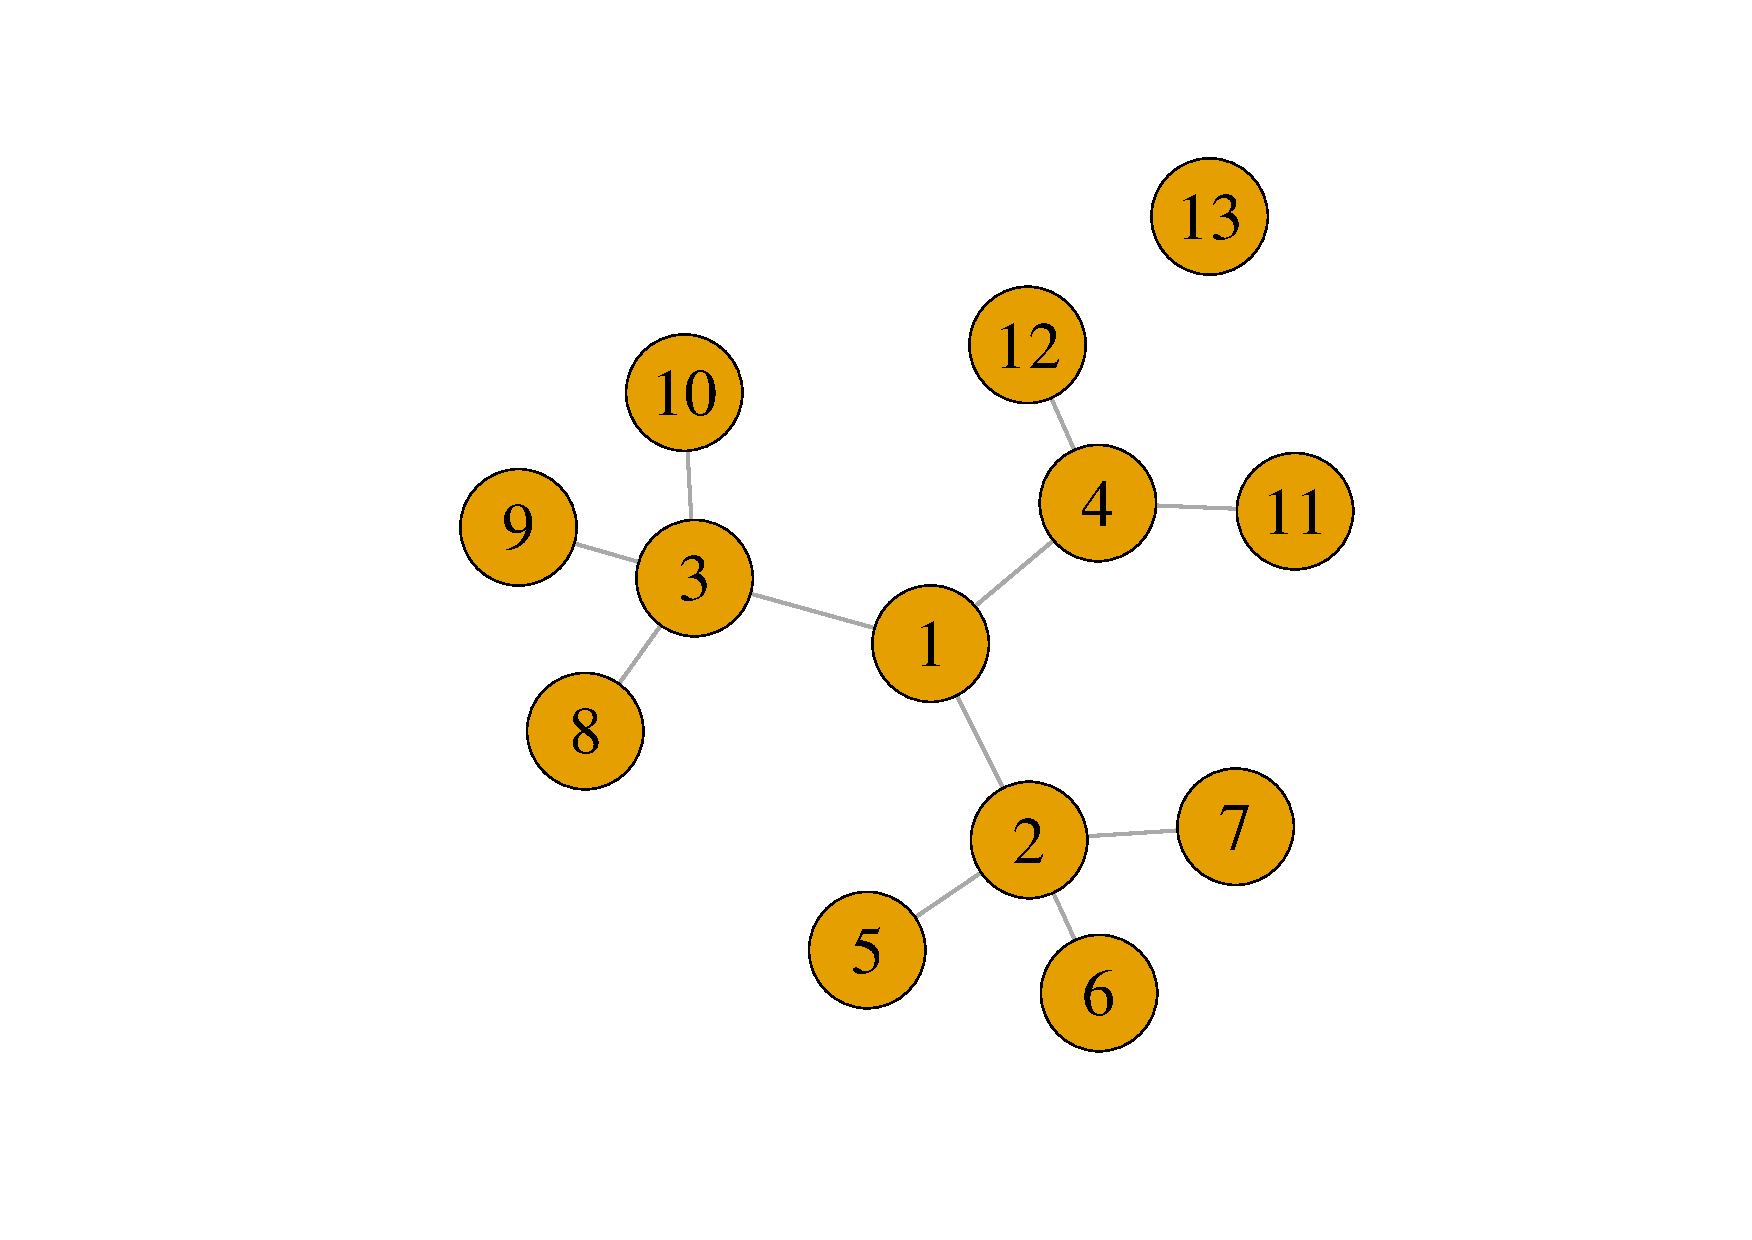
\includegraphics[scale=0.20]{figures/conteg.pdf}
%\end{column}
%\hspace*{0.2cm}\begin{column}{0.5\textwidth}
%\begin{itemize}
%\begin{tiny}
%\color{isegreen}
%\item degree centrality: node 1 has centrality 3, node 2 and 3 have centrality 4, node 4 has centrality 3;
%\item closeness centrality: node 1 has centrality 0.63, node 2 and 3 have centrality 0.52, node 4 has centrality 0.48;
%\item betweenness centrality: node 1 has centrality 0.61, node 2 and 3 have centrality 0.36, node 4 has centrality 0.27;
%\item eigenvector centrality: node 1 has centrality 0.51, node 2 and 3 have centrality 0.44, node 4 has centrality 0.33;
%\end{tiny}
%\end{itemize}
%\end{column}
%\end{columns}
%Conclusion: Node 1 is the central node by all centrality measures but degree centrality;
%Node 2 and 3 are central nodes by degree centrality
%}
%

\frame{
\frametitle{Minnesota Road Networks}
\begin{itemize}
\item Minnesota Road Net data \textcolor{purple}{minnesota.mat} is avaiable in Matlab R2016b and later versions
\item Minnesota State of United States
\item The data contains a $G$ object which is a combination of Nodes (Coordinates of locations) and Edges (roads between each pair of nodes)
\end{itemize}
}

\frame{
\frametitle{Minnesota Road Networks}
\begin{figure}
\begin{tabular}{cc}
\subfloat{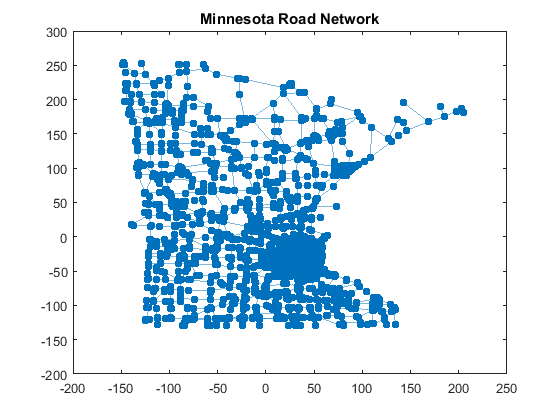
\includegraphics[scale=0.35]{figures/minnesotaroadnet.png}}
&\subfloat{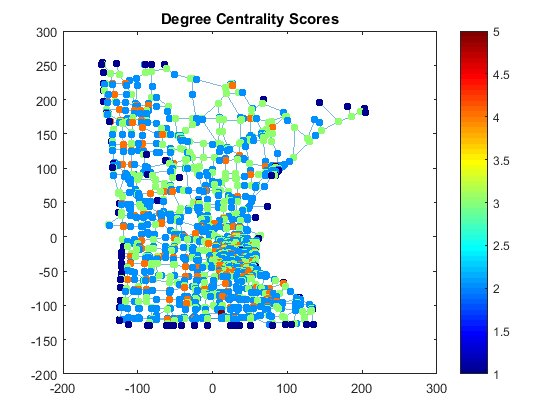
\includegraphics[scale=0.35]{figures/degreecentr.png}}
\end{tabular}
\vspace{-0.5cm}
\caption{Display of Minnesota Road Net -- no centrality displayed (left), degree centrality $C_{D}$ (right)}
\vspace{-0.2cm}
    \href{https://github.com/QuantLet/METISNET/tree/master/METISNET-centralitycomparison}{\quantnet METISNET-centralitycomparison}
\end{figure}
}

\frame{
\frametitle{Minnesota Road Networks}
\begin{figure}
\begin{tabular}{cc}
\subfloat{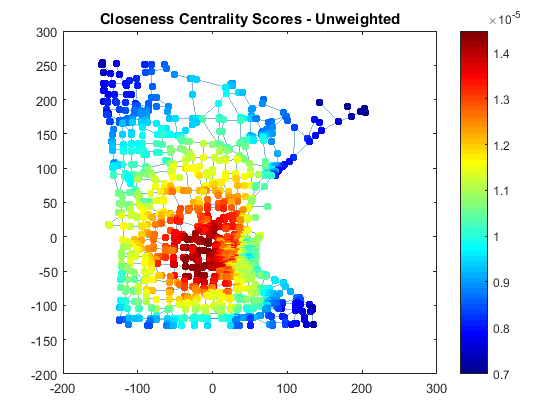
\includegraphics[scale=0.35]{figures/closeness_unweighted.png}}
&\subfloat{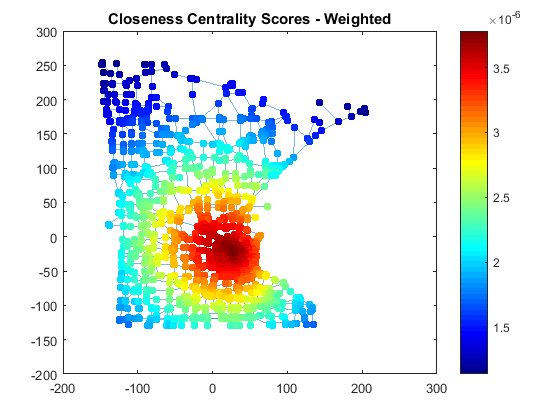
\includegraphics[scale=0.35]{figures/closeness_weighted.png}}
\end{tabular}
\vspace{-0.5cm}
\caption{Display of Minnesota Road Net -- closeness centrality unweighted (left), closeness centrality weighted (right)}
\vspace{-0.2cm}
    \href{https://github.com/QuantLet/METISNET/tree/master/METISNET-centralitycomparison}{\quantnet METISNET-centralitycomparison}
\end{figure}
}

\frame{
\frametitle{Minnesota Road Networks}
\begin{figure}
\begin{tabular}{cc}
\subfloat{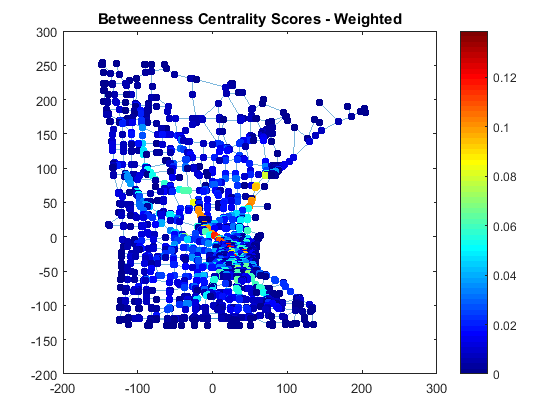
\includegraphics[scale=0.35]{figures/btwness_unweighted.png}}
&\subfloat{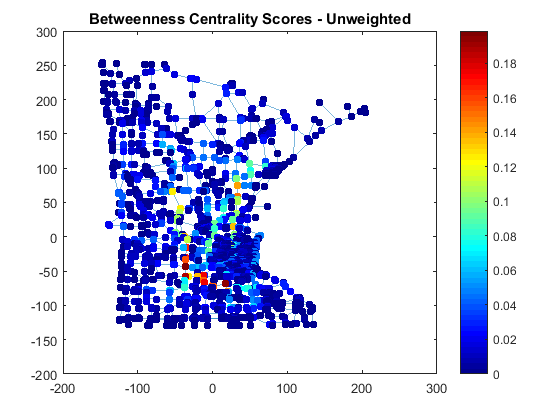
\includegraphics[scale=0.35]{figures/btwness_weighted.png}}
\end{tabular}
\vspace{-0.5cm}
\caption{Display of Minnesota Road Net -- betweenness centrality unweighted (left), betweenness centrality weighted (right)}
\vspace{-0.2cm}
    \href{https://github.com/QuantLet/METISNET/tree/master/METISNET-centralitycomparison}{\quantnet METISNET-centralitycomparison}
\end{figure}
}

\frame{
\frametitle{Minnesota Road Networks}
\begin{figure}
\begin{tabular}{cc}
\subfloat{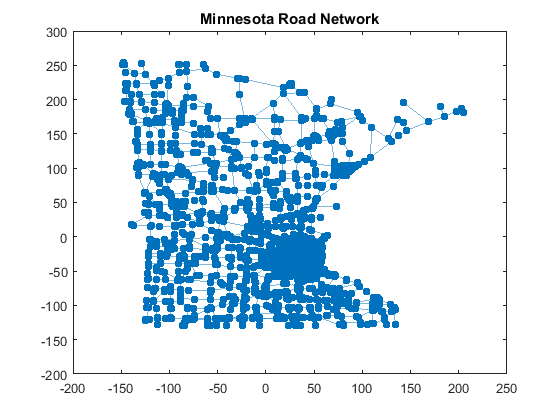
\includegraphics[scale=0.35]{figures/minnesotaroadnet.png}}
&\subfloat{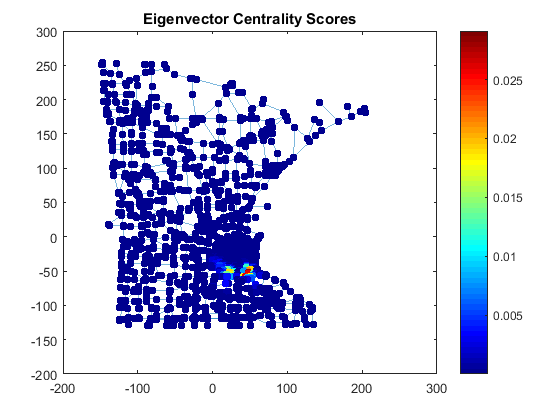
\includegraphics[scale=0.35]{figures/eigenctr.png}}
\end{tabular}
\vspace{-0.2cm}
\caption{Display of Minnesota Road Net -- no centrality displayed (left), eigenvector centrality $C_{E}$(right)}
\vspace{-0.5cm}
    \href{https://github.com/QuantLet/METISNET/tree/master/METISNET-centralitycomparison}{\quantnet METISNET-centralitycomparison}
\end{figure}
}
%%%%%%%%%%%%%%%%%%%%%%%%%%%%%%%%%
\section{Extension: Directed Cases}
\frame{
\frametitle{Notation \& Terminology}
A \textbf{directed graph} $\mathcal{G}=(\mathcal{V},\mathcal{E})$ consists of a list of vertices $\mathcal{V}=\{1,2,\ldots, N\}$ \,and a set of \textbf{ordered edges} $\mathcal{E} = \{(i,j), (j,i), (k, l),(l, k) \ldots\}$ for $i, j, k, l \in \mathcal{V}$
where
\bigskip{}
\begin{itemize}
\item vertices $\mathcal{V}$: node, individual, agent,
\bigskip
\item edges $\mathcal{E}$: arrows, directed edges, directed lines.
\end{itemize}
}

\frame{
\frametitle{Notation \& Terminology}
A \textbf{directed graph} could be represented by its \textbf{adjacency matrix} $A = [a_{i,j}]$ where
\begin{displaymath}
 a_{i, j} = \left\{\begin{array}{ll}
 1 &  \textrm{if there is an arrow from i to j}\\
 0 & otherwise \\
 \end{array} \right.
 \end{displaymath}
\begin{itemize}
\item there is no need to be an arrow from j to i simutaneouly.
\end{itemize}
}

\frame{
\frametitle{Degree Centrality: Directed Cases}
The \textbf{in-degree centrality} of node $v_{k}$  is given by:
\textcolor{iseblue}{$$C_{InD}(v_{k}) = \sum_{i=1}^n a_{(v_{i},v_{k})}$$ }
\begin{itemize}
\item $ a(v_{i},v_{k})$ equals 1 , if there is an arrow from $v_{i}$ to $v_{k}$ and 0 otherwise.
\end{itemize}
\smallskip
The \textbf{out-degree centrality} of node $v_{k}$ is given by:
\textcolor{iseblue}{$$C_{OutD}(v_{k}) = \sum_{i=1}^n a_{(v_{k},v_{i})}$$ }
\begin{itemize}
\item $ a(v_{k},v_{i})$ equals 1 , if there is an arrow from $v_{k}$ to $v_{i}$ and 0 otherwise.
\end{itemize}
}


\begin{frame}	
\frametitle{Example:}
\color{isegreen}
\textbf{Degree Centrality: Directed Cases}
\color{iseblue}
\begin{columns}[onlytextwidth]
\hspace{-0.5 cm}
\begin{column}{0.5\textwidth}
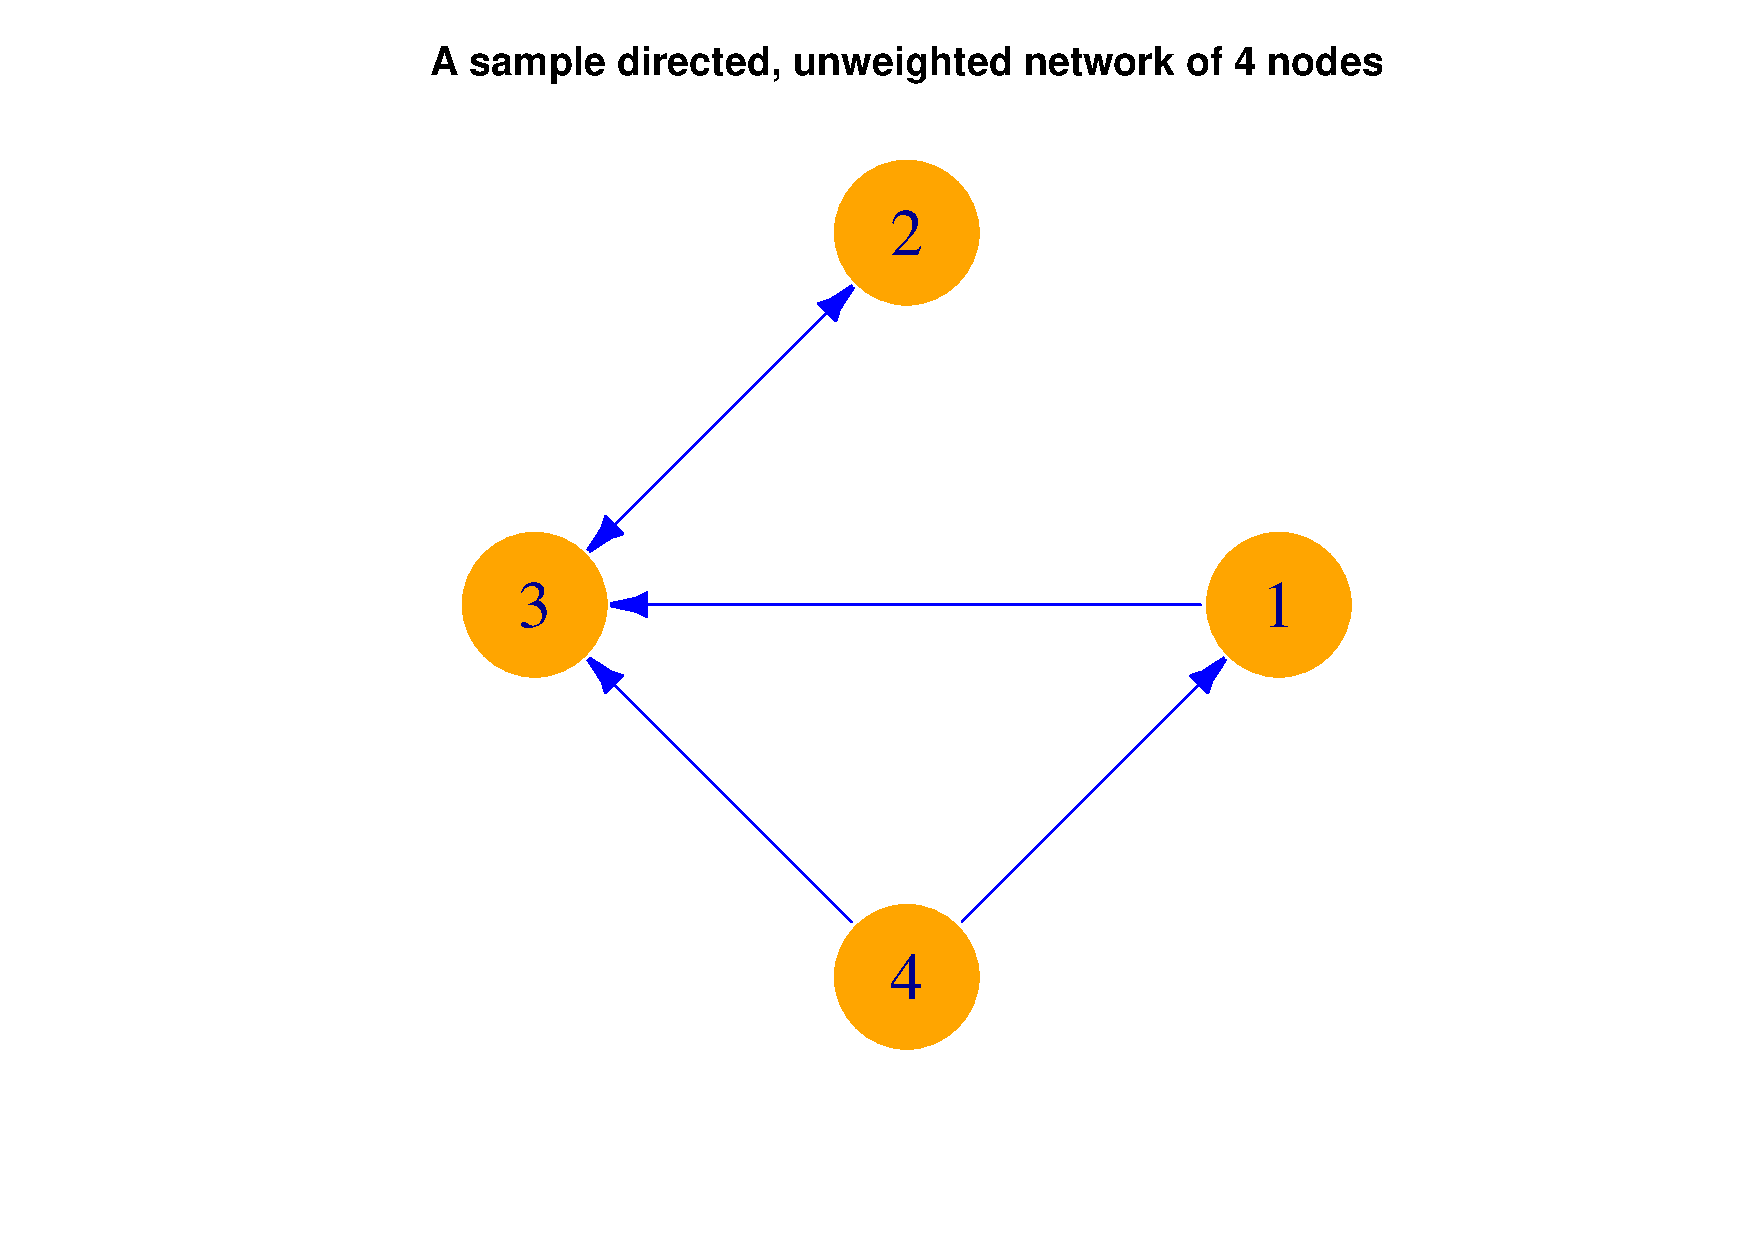
\includegraphics[scale=0.25]{figures/4ndirected.pdf}
\end{column}
\hspace*{0.2cm}\begin{column}{0.5\textwidth}
\begin{itemize}
\begin{small}
\color{isegreen}
\item $C_{InD}(1) =C_{InD}(2)  = 1, C_{InD}(3)  = 3,C_{InD}(4)  = 0 $
\item $C_{OutD}(1) = C_{OutD}(2)=1, C_{OutD}(3)=0, C_{OutD}(4) = 2 $
\end{small}
\end{itemize}
\end{column}
\end{columns}
\end{frame}

\frame{
\frametitle{Katz Centrality}
The Katz centrality of node $v_{k}$ is given by:
\textcolor{iseblue}{$$C_{K}(v_{k}) = \alpha \sum_{i=1}^n a_{(v_{i},v_{k})} \, C_{K}(v_{i}) + \beta$$ }
\begin{itemize}
\item $\alpha$ : scaling vector to normalize the score
\item $\beta$ : weight of the centrality of vertices ego is tied to .
  \begin{itemize}
  \item if $\beta > 0 $, ego has higher centrality when tied to vertices that are central
  \item if $\beta < 0 $, ego has higher centrality when tied to vertices that are not central
   \item with $\beta = 0 $, it is degree centrality
\end{itemize}
\end{itemize}
}


\frame{
In matrix form : 
\textcolor{iseblue}{$$C_{K} = \alpha C_{K} A + \beta$$}
\begin{itemize}
\item where $\beta$ is now a vector whose elements are all equal a given positive constant.
\end{itemize}
}

\frame{
It follows that $C_{K}$ can be computed as:
\textcolor{iseblue}{$$C_{K} = \beta (I - \alpha A)^{-1} $$}
\begin{itemize}
\item The Katz status of a node is defined as the number of weighted paths reaching the node in the network plus an exogenous factor, a generalization of the in-degree measure which counts only paths of length one.
\end{itemize}
}

\frame{
\frametitle{PageRank Centrality}
The PageRank centrality of node $v_{k}$ is given by:
\textcolor{iseblue}{$$C_{PR}(v_{k}) = \alpha \sum_{i=1}^n \frac{a_{k,i}}{d(v_{i})} \, C_{PR}(v_{i}) + \beta$$ }
\begin{itemize}
\item $\alpha$ and $\beta$ are constants
\item $d(v_{i})$ is the out-degree of node $v_{i}$ if such degree is positive, or $d(v_{i})=1$ if the out-degree of $v_{i}$ is null.
\end{itemize}
}

\frame{
In matrix form :
\textcolor{iseblue}{$$C_{PR} = \alpha C_{PR} D^{-1}A + \beta$$ }
\begin{itemize}
\item $\beta$ is now a vector whose elements are all equal a given positive constant
\item $D^{-1}$ is a diagonal matrix with $i$-th diagonal element equal to $1/d(v_{i})$.
\end{itemize}
}

\frame{
It follows that $C_{PR}$ can be computed as:
\textcolor{iseblue}{$$C_{PR} = \beta (I - \alpha D^{-1}A)^{-1}$$}
\begin{itemize}
\item The damping factor $\alpha$ and the personalization vector $\beta$ have the same role seen for Katz centrality.
\end{itemize}
}



%%%%%%%%%%%%%%%%%%%%%%%%%%%%%%%%%%%%%
\section{Graph Centrality}
\begin{frame}
\frametitle{Two Certain Features of Graph Centralization}
\begin{itemize}
	\item It should index the degree to which the centrality of the most central node exceeds the centrality of all other nodes
	\item It should each be expressed as a ratio of that excess to its maximum possible value for a graph containing the observed number of nodes. 
\end{itemize}	
\end{frame}

\begin{frame}
Then Freeman(1977) proposed a measure in graph centrality.
\color{iseblue}
\begin{equation}
C_X=\frac{\sum_{i=1}^n\{C_X(v^*)-C_X(v_i)\}}{\max\sum_{i=1}^n\{C_X(v^*)-C_X(v_i)\}}	
\end{equation}
\begin{itemize}
	\item $n$: number of nodes
	\item $C_X(v_i)$: one of the nodes centralities defined above
	\item $C_X(v^*)$: largest value of $Cx(v_i)$ for any node in the network
	\item $\max \sum_{i=1}^n\{C_X(v^*)-C_X(v_i)\}$: the maximum possible sum of differences in node centrality for a graph of n nodes
\end{itemize}		
\end{frame}


\begin{frame}
\frametitle{Degree-based measures of graph centrality}
\color{iseblue}	
\begin{eqnarray*}
	C_D &=&\frac{\sum_{i=1}^n\{C_D(v^*)-C_D(v_i)\}}{\max\sum_{i=1}^n\{C_D(v^*)-C_D(v_i)\}} \\
	 &=& \frac{\sum_{i=1}^n\{C_D(v^*)-C_D(v_i)\}}{n^2-3n+2}\\
\end{eqnarray*}
\end{frame}

\begin{frame}
	\frametitle{Betweeness-based measures of graph centrality}
	\color{iseblue}
	\begin{eqnarray*}
		C_B &=& \frac{2\sum_{i=1}^n\{C_B'(v^*)-C_B'(v_i)\}}{n-1}\\
		&=& \frac{\sum_{i=1}^n\{C_B(v^*)-C_B(v_i)\}}{n^3-4n^2+5n-2}\\
	\end{eqnarray*}
\end{frame}

\begin{frame}
	\frametitle{Closeness-based measures of graph centrality}
	\color{iseblue}
	\begin{eqnarray*}
		C_C = \frac{\sum_{i=1}^n\{C_C'(v^*)-C_C'(v_i)\}}{(n^2-3n+2)/(2n-3)}\\
	\end{eqnarray*}
\end{frame}

%%%%%%%%%%%%%%%%%%%%%%%%%%%%%%%%%%%%%%%%%%%%%%%%%%%%%%%
\section{Examples of Various Graph Centralities}
\begin{frame}	
\frametitle{Example:}
\color{isegreen}
\textbf{Degree Centrality}
\color{iseblue}
\begin{columns}[onlytextwidth]
\hspace{-0.5 cm}
\begin{column}{0.5\textwidth}
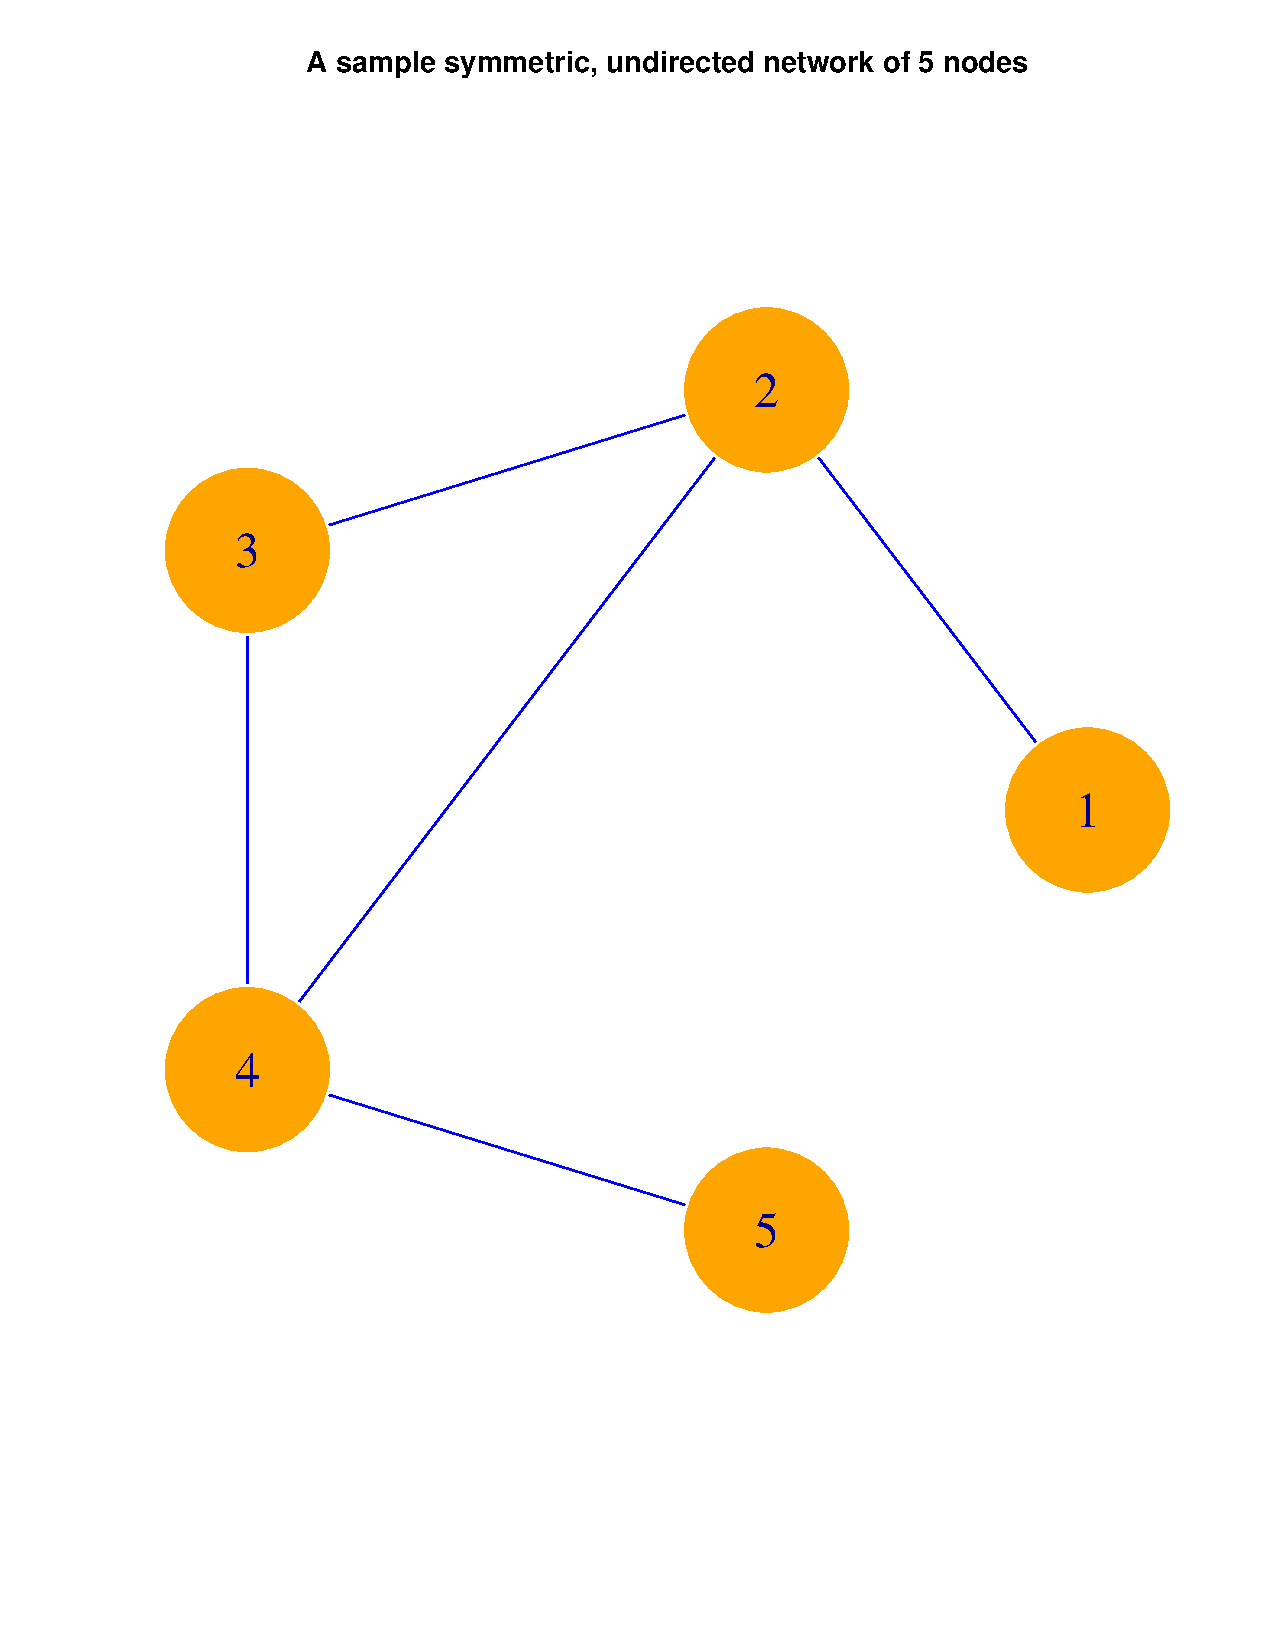
\includegraphics[scale=0.25]{picture1.pdf}
\end{column}
\hspace*{0.2cm}\begin{column}{0.5\textwidth}
\begin{itemize}
\begin{small}
\color{isegreen}
\item $C_D=0.42$
\item $C_D(v_1)=1$,$C_D(v_2)=3$,$C_D(v_3)=2$,$C_D(v_4)=3$,$C_D(v_5)=1$;
\item $C_D'(v_1)=0.25$,$C_D'(v_2)=0.75$,$C_D'(v_3)=0.5$,$C_D'(v_4)=0.75$,$C_D'(v_5)=0.25$
\end{small}
\end{itemize}
\end{column}
\end{columns}
\end{frame}

\begin{frame}	
\color{isegreen}
\textbf{ Betweenness Centrality}
\color{iseblue}
\begin{columns}[onlytextwidth]
\hspace{-0.5 cm}
\begin{column}{0.5\textwidth}
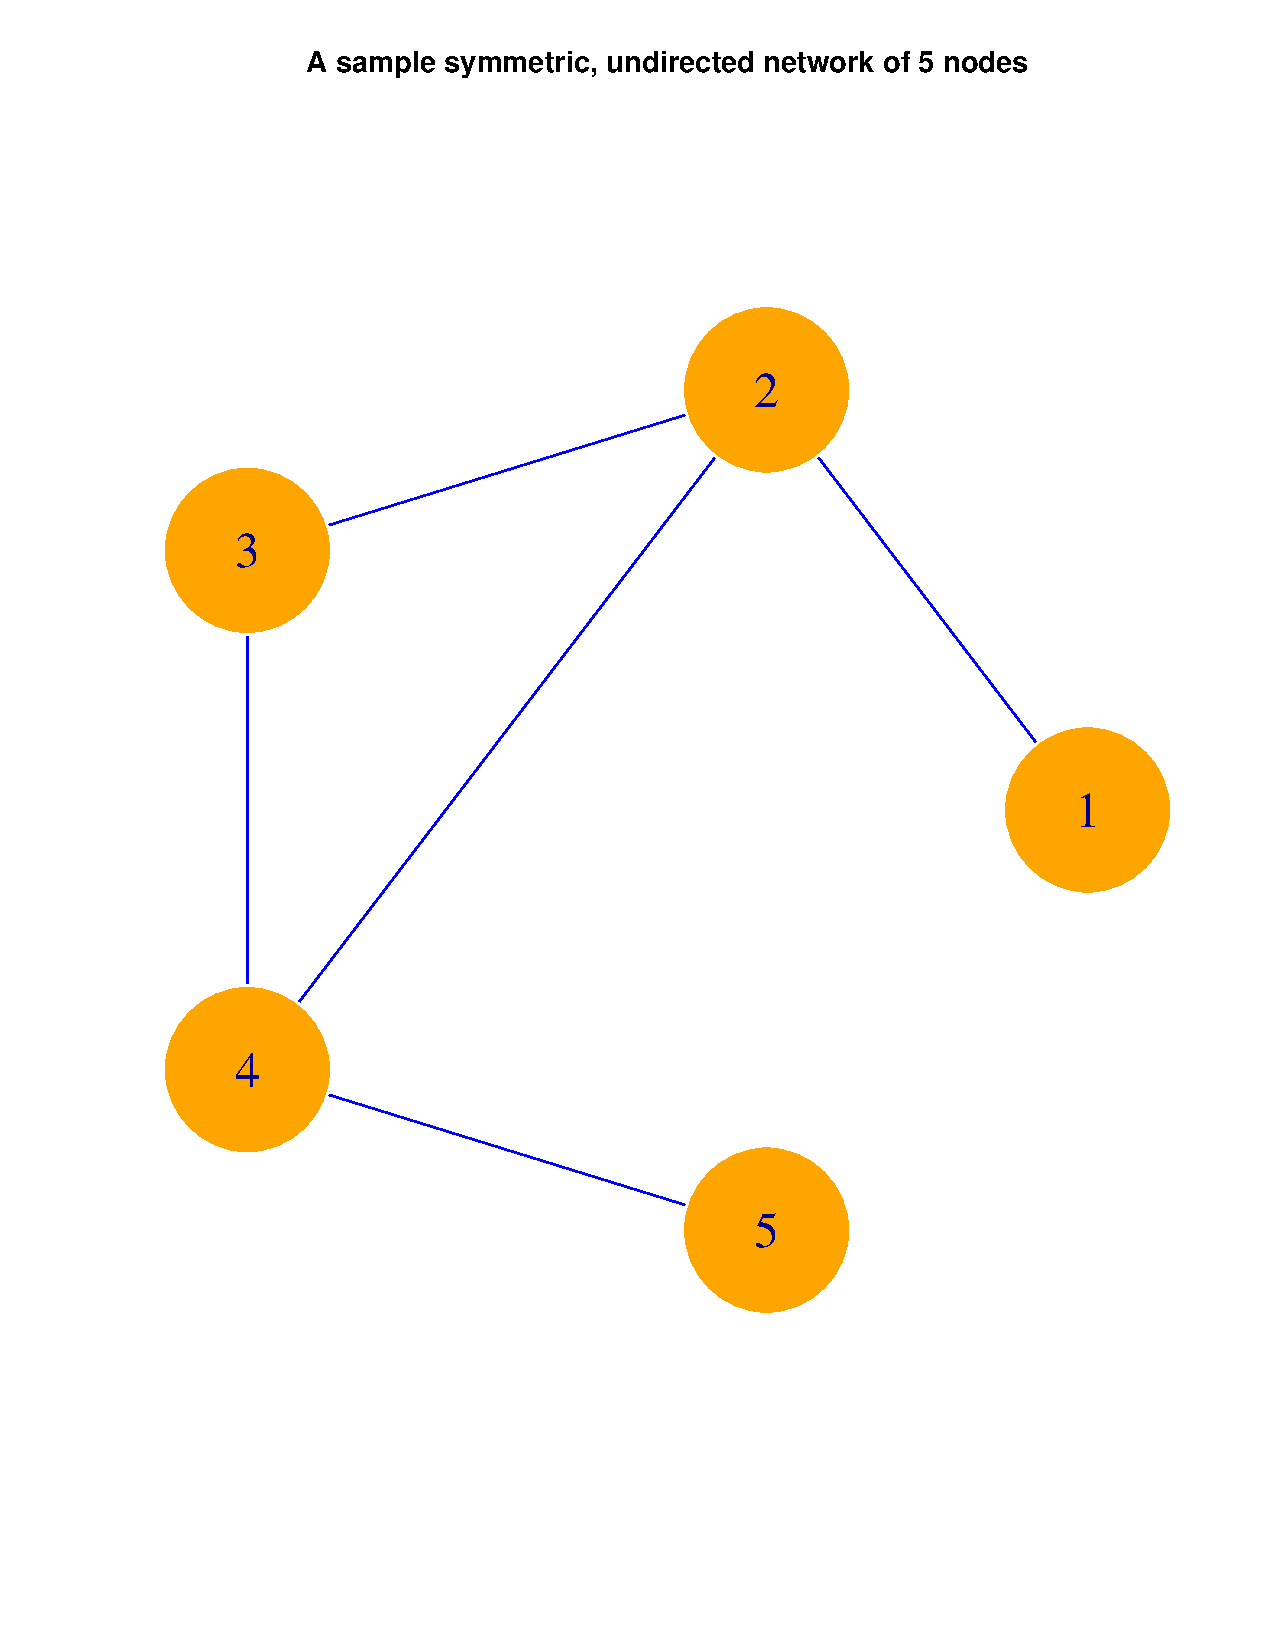
\includegraphics[scale=0.25]{picture1.pdf}
\end{column}
\hspace*{0.2cm}\begin{column}{0.5\textwidth}
\begin{itemize}
\begin{small}
\color{isegreen}
\item $C_B=0.38$
\item $C_B(v_1)=0$,$C_B(v_2)=3$,$C_B(v_3)=0$,$C_B(v_4)=3$,$C_B(v_5)=0$;
\item $C_B'(v_1)=0$,$C_B'(v_2)=0.5$,$C_B'(v_3)=0$,$C_B'(v_4)=0.5$,$C_B'(v_5)=0$
\end{small}
\end{itemize}
\end{column}
\end{columns}
\end{frame}

\begin{frame}	
\color{isegreen}
\textbf{Closeness Centrality}
\color{iseblue}
\begin{columns}[onlytextwidth]
\hspace{-0.5 cm}
\begin{column}{0.5\textwidth}
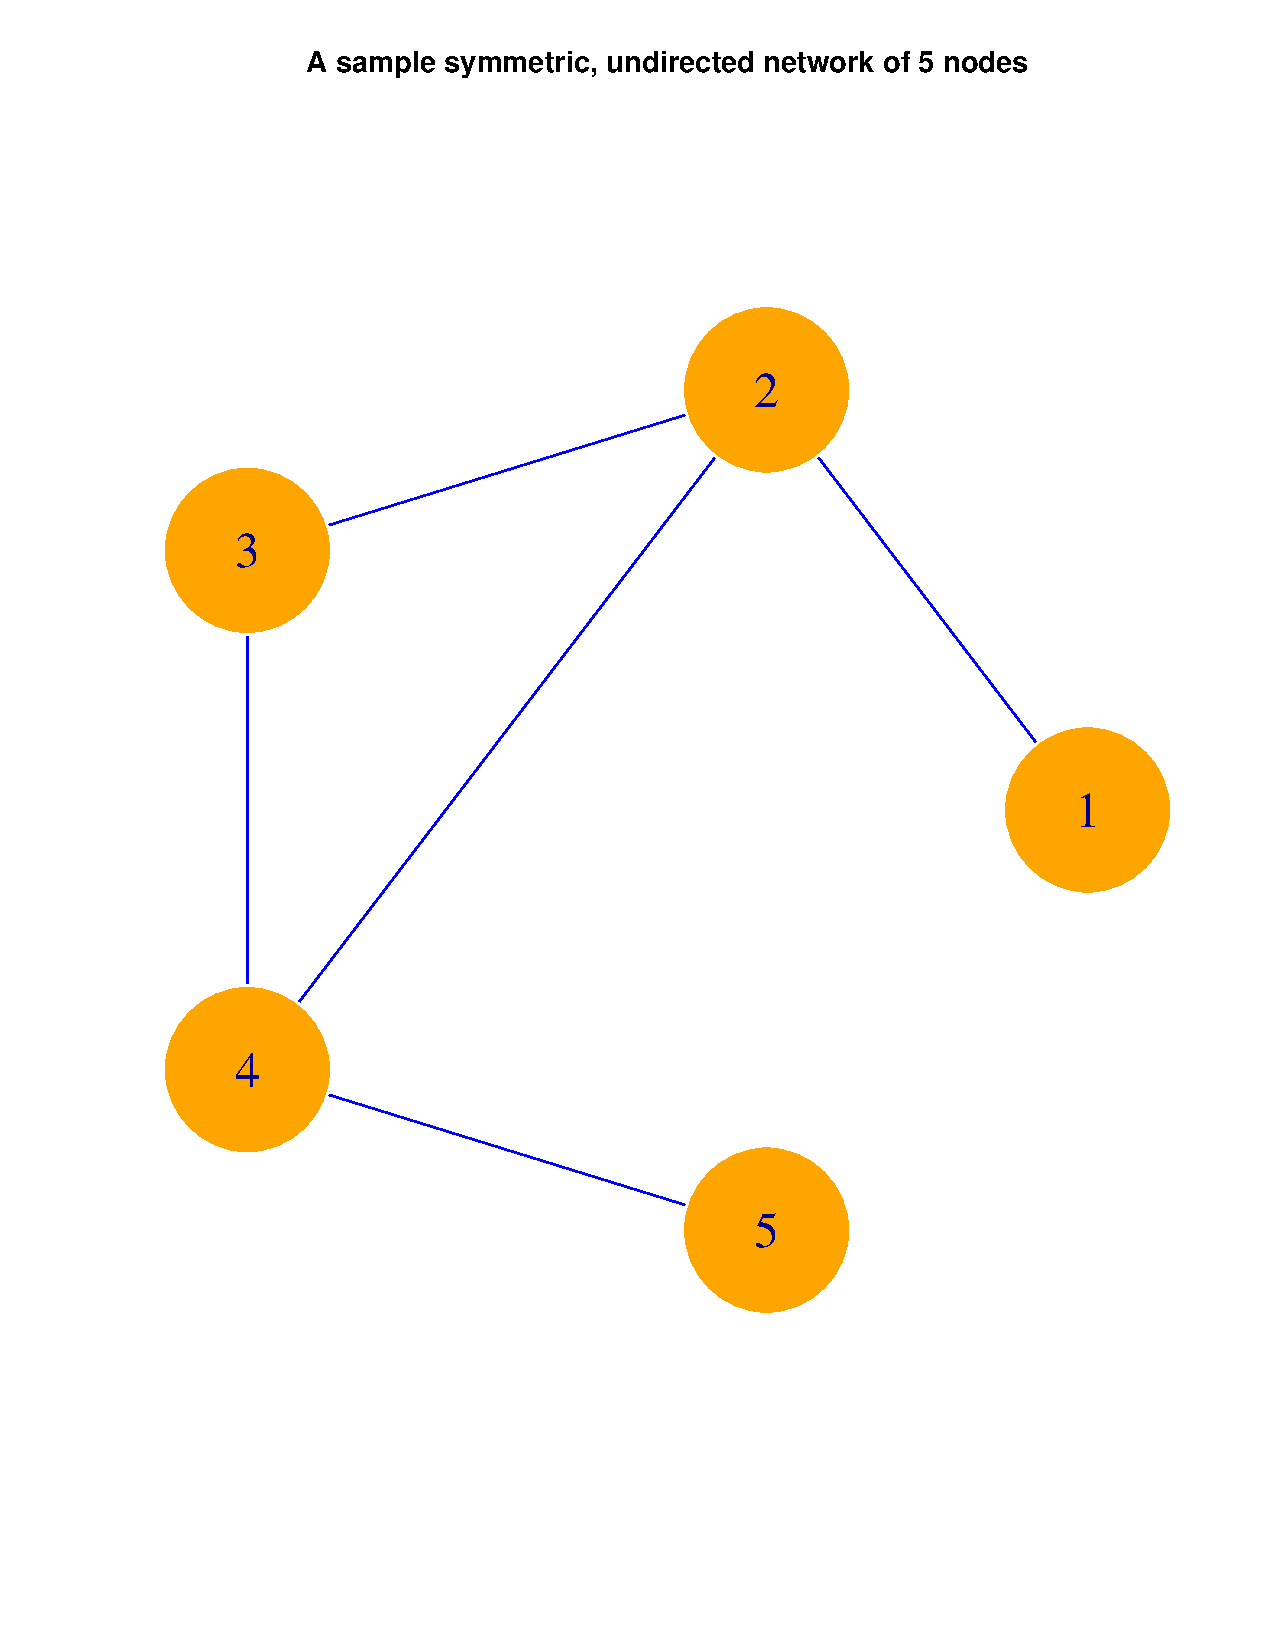
\includegraphics[scale=0.25]{picture1.pdf}
\end{column}
\hspace*{0.2cm}\begin{column}{0.5\textwidth}
\begin{itemize}
\begin{small}
\color{isegreen}
\item $C_C=0.43$
\item $C_C(v_1)^{-1}=8$,$C_C(v_2)^{-1}=5$,$C_C(v_3)^{-1}=6$,$C_C(v_4)^{-1}=5$,$C_C(v_5)^{-1}=8$;
\item $C_C'(v_1)=0.5$,$C_C'(v_2)=0.8$,$C_C'(v_3)=0.67$,$C_C'(v_4)=0.8$,$C_C'(v_5)=0.5$
\end{small}
\end{itemize}
\end{column}
\end{columns}
\end{frame}


\section{Reference}
%%%%%%%%%%%%%%%%%%%%%%%%%%%%%%%%%%%%%%%%%%%%%%%%%%%%%%%%%%%%%%%%%%%%%%%%%%%%%%%%%%%%%%%%%%%%%%%%%%%%%%%%%%%%%%%%%%%%%%%%
\frame{
\frametitle{Reference}
\begin{thebibliography}{aaaaaaaaaaaaaaaaa}
\beamertemplatearticlebibitems
\bibitem{Anthonisse:1971}
Anthonisse, J. M.
\newblock{\em The Rush in a Graph}
\newblock Mathematisch Centrum, Amsterdam, 1971.
\beamertemplatearticlebibitems
\bibitem{Bavelas, A. :1950}
Bavelas, A.
\newblock{\em Communication patterns in task oriented groups}
\newblock Journal of the Acoustical Society of America, 22:271-282, 1950.
\beamertemplatearticlebibitems
\bibitem{Beauchamp, M. A.:1965}
Beauchamp, M. A.
\newblock{\em An improved index of centrality}
\newblock BehavioralScience, 10:161-163, 1965.
\end{thebibliography}
}

\frame{
\frametitle{Reference}
\begin{thebibliography}{aaaaaaaaaaaaaaaaa}
\beamertemplatearticlebibitems
\bibitem{Moxley, R. L. and N. F. Moxley :1974}
Moxley, R. L. and N. F. Moxley
\newblock{\em Determining point-centrity in uncontrived social networks}
\newblock Sociometry, 37:122-130,1974.
\beamertemplatearticlebibitems
\bibitem{Nieminen, J. :1974}
Nieminen, J.
\newblock{\em On centrality in a graph}
\newblock Scandinavian Journal of Psychology, 15:322-336, 1974.
\beamertemplatearticlebibitems
\bibitem{Rogers, D. L. :1974}
Rogers, D. L.
\newblock{\em Sociometric analysis of interorganizational relations: application of theory and measurement}
\newblock Rural Sociology, 39:487-503, 1974.
\end{thebibliography}
}

\frame{
\frametitle{Reference}
\begin{thebibliography}{aaaaaaaaaaaaaaaaa}
\beamertemplatearticlebibitems
\bibitem{Shaw, M. E. :1954}
Shaw, M. E.
\newblock{\em Group structure and the behavior of individuals in small groups}
\newblock Journal Of Psychology, 38: 139-149, 1954.
\beamertemplatearticlebibitems
\bibitem{Sabidussi, G. :1966}
Sabidussi, G.
\newblock{\em The centrality index of a graph}
\newblock Psychomatrika, 31 581-603, 1966.
\beamertemplatearticlebibitems
\bibitem{Freeman L. C.:1977}
Rogers, D. L.
\newblock{\em A set of measures of centrality based on betweenness}
\newblock Sociometry, 40:3541, 1977.
\end{thebibliography}
}


\frame[plain]{
\titlepage
}
\end{document}